\chapter{Resultados} \label{resultados}

Neste capítulo são detalhados os resultados obtidos em cada fase do processo de
KDD aplicado neste trabalho. Ele está nas mesmas seções do capítulo anterior,
pois cada fase do KDD contribui para o resultado final do processo e gera seus
próprios conhecimentos.

\section{Entrada de dados}

Para a etapa de entrada de dados, foram desenvolvidos \textit{scripts} em SQL
que criavam tabelas na base de dados em MySQL com subconjuntos de dados
relacionados com os cursos selecionados para esse estudo. Esses \textit{scripts}
estão disponíveis no Apêndice \ref{anex:anexo1}. O Quadro \ref{reducedDataTables}
apresenta e resume essas tabelas auxiliares.

\begin{quadro}[!htb]
  \centering
  \caption{Descrição das tabelas criadas apenas com dados dos cursos selecionados}
  \label{reducedDataTables}
  \begin{tabular}{|l|l|}
    \hline
    \multicolumn{1}{|c|}{\textbf{Tabela}} & \multicolumn{1}{c|}{\textbf{Descrição}} \\ \hline
    \textit{adm} & \begin{tabular}[c]{@{}l@{}}Tabela base agrupando dados de cada aluno do curso \\ Bacharelado em Administração Pública em cada \\ disciplina em que ele cursou.\end{tabular} \\ \hline
    \textit{adm\_base\_log\_reduzido} & \begin{tabular}[c]{@{}l@{}}Tabela com registros de log dos alunos e cursos do curso\\ Bacharelado em Administração Pública.\end{tabular} \\ \hline
    \textit{adm\_disciplinas} & \begin{tabular}[c]{@{}l@{}}Registra o identificador das disciplinas do curso de\\ Bacharelado em Administração Pública, data de início \\ e data de fim.\end{tabular} \\ \hline
    \textit{adm\_id\_alunos} & \begin{tabular}[c]{@{}l@{}}Registra o identificador dos alunos matriculados no \\ curso de Bacharelado em Administração Pública.\end{tabular} \\ \hline
    \textit{lic\_ped} & \begin{tabular}[c]{@{}l@{}}Tabela base agrupando dados de cada aluno do curso \\ Licenciatura em Pedagogia em cada disciplina\\ em que ele cursou.\end{tabular} \\ \hline
    \textit{lic\_ped\_base\_log\_reduzido} & \begin{tabular}[c]{@{}l@{}}Tabela com registros de log dos alunos e cursos do curso\\ Licenciatura em Pedagogia.\end{tabular} \\ \hline
    \textit{lic\_ped\_disciplinas} & \begin{tabular}[c]{@{}l@{}}Registra o identificador das disciplinas do curso de\\ Licenciatura  em Pedagogia, data de início e data de fim.\end{tabular} \\ \hline
    \textit{lic\_ped\_id\_alunos} & \begin{tabular}[c]{@{}l@{}}Registra o identificador dos alunos matriculados no\\  curso de Licenciatura em Pedagogia.\end{tabular} \\ \hline
  \end{tabular}
  \Ididthis
\end{quadro}

Essas tabelas se tornaram necessárias, pois, executar \textit{scripts} que
buscassem dados em toda a base do Moodle demandava horas de processamento. Em
contrapartida, utilizando apenas essas tabelas o tempo de execução foi reduzido
para poucos minutos.

\section{Pré-processamento}

Utilizando as tabelas do Quadro \ref{reducedDataTables} e os \textit{scripts}
disponíveis no Apêndice \ref{anex:anexo1}, as variáveis, mapeadas para construtos
da TDT por \citeonline{ramos2016abordagem} foram salvas como valores separados
por vígulas (CSV) em uma tabela cujas colunas eram os identificadores listados
no Quadro \ref{variablesDescritionTable}.

\begin{center}
\renewcommand\LTcaptype{quadro}
\begin{longtable}[c]{|l|l|l|}
  \caption{Lista das variáveis e respectivos construtos e seus identificadores}
  \label{variablesDescritionTable}\\
  \hline
  \multicolumn{1}{|c|}{\textbf{Identificador}} & \multicolumn{1}{c|}{\textbf{Variáveis}} & \multicolumn{1}{c|}{\textbf{Construto}} \\ \hline
  \endfirsthead
  %
  \multicolumn{3}{c}%
  {{\bfseries Quadro \thequadro\ continuação da página anterior}} \\
  \hline
  \multicolumn{1}{|c|}{\textbf{Identificador}} & \multicolumn{1}{c|}{\textbf{Variáveis}} & \multicolumn{1}{c|}{\textbf{Construto}} \\ \hline
  \endhead
  %
  VAR01 & \begin{tabular}[c]{@{}l@{}}Quantidade geral de postagens do aluno em fóruns,\\ por disciplina.\end{tabular} & Diálogo \\ \hline
  VAR02 & \begin{tabular}[c]{@{}l@{}}Quantidade geral de mensagens enviadas pelo\\ aluno dentro do ambiente, por semestre.\end{tabular} & Diálogo \\ \hline
  VAR03 & \begin{tabular}[c]{@{}l@{}}Quantidade geral de mensagens recebidas pelo\\ aluno dentro do ambiente, por semestre.\end{tabular} & Diálogo \\ \hline
  VAR04 & \begin{tabular}[c]{@{}l@{}}Quantidade geral de recursos disponibilizados pelo\\ professor (página web, vídeo, pdfs, entre outros)\\ por disciplina.\end{tabular} & Estrutura \\ \hline
  VAR05a & \begin{tabular}[c]{@{}l@{}}Quantidade de acessos do aluno ao ambiente por\\ turno (Manhã), por semestre.\end{tabular} & Autonomia \\ \hline
  VAR05b & \begin{tabular}[c]{@{}l@{}}Quantidade de acessos do aluno ao ambiente por\\ turno (Tarde), por semestre.\end{tabular} & Autonomia \\ \hline
  VAR05c & \begin{tabular}[c]{@{}l@{}}Quantidade de acessos do aluno ao ambiente por\\ turno (Noite), por semestre.\end{tabular} & Autonomia \\ \hline
  VAR06 & \begin{tabular}[c]{@{}l@{}}Quantidade de colegas diferentes para quem o\\ aluno enviou mensagens no ambiente, por\\ semestre.\end{tabular} & Diálogo \\ \hline
  VAR07 & \begin{tabular}[c]{@{}l@{}}Quantidade de acessos do aluno ao ambiente no\\ semestre.\end{tabular} & Autonomia \\ \hline
  VAR08 & \begin{tabular}[c]{@{}l@{}}Quantidade de mensagens enviadas pelo aluno\\ aos professores pelo ambiente, por semestre.\end{tabular} & Diálogo \\ \hline
  VAR09 & \begin{tabular}[c]{@{}l@{}}Quantidade de mensagens dos professores recebidas\\ pelo aluno no ambiente, por semestre.\end{tabular} & Diálogo \\ \hline
  VAR10 & \begin{tabular}[c]{@{}l@{}}Quantidade de mensagens de colegas recebidas pelo\\ aluno no ambiente, por semestre.\end{tabular} & Diálogo \\ \hline
  VAR11 & \begin{tabular}[c]{@{}l@{}}Quantidade de mensagens enviadas pelo aluno para\\ outros colegas no ambiente, por semestre.\end{tabular} & Diálogo \\ \hline
  VAR12 & \begin{tabular}[c]{@{}l@{}}Quantidade de atividades com prazos de resposta ou\\ envio definidos por professor, por disciplina.\end{tabular} & Estrutura \\ \hline
  VAR13 & \begin{tabular}[c]{@{}l@{}}Quantidade de acessos do aluno aos diferentes tipos\\ de atividades disponibilizadas (webquest, fórum,\\ quiz, entre outros), por disciplina.\end{tabular} & Autonomia \\ \hline
  VAR14 & \begin{tabular}[c]{@{}l@{}}Quantidade de fóruns de discussão disponibilizados\\ sobre os conteúdos por disciplina.\end{tabular} & Estrutura \\ \hline
  VAR15 & \begin{tabular}[c]{@{}l@{}}Quantidade de acessos do aluno aos fóruns, por\\ disciplina.\end{tabular} & Autonomia \\ \hline
\end{longtable}
\Otherguydidthis{ramos2016abordagem}
\end{center}

Além das variáveis, cada linha possui o identificador de um aluno e de uma
disciplina. Dessa forma, cada linha representa um aluno em uma disciplina do
curso.

Essas tabelas foram convertidas para planilhas eletrônicas para facilitar o
processo de correção e validação dos resultados. As planilhas serviram como base
para os processos de mineração de dados.

\section{Mineração de Dados}

As planilhas eletrônicas foram carregadas em \textit{dataframes}, como foi
descrito no capítulo \ref{metodos}.

Os dados do curso de Licenciatura em Pedagogia somaram 6240 entradas. Sendo que,
$50,6\%$ foram marcados como não evadidos e $49,4\%$ foram marcados como
evadido, como ilustra a Figura \ref{classDistribuitionPedTotal}. A proporção das
classes após a divisão dos dados em conjunto de testes e conjunto de treinamento
é mostrada nas Figuras \ref{classDistribuitionPedTest} e
\ref{classDistribuitionPedTrain}, respectivamente.

\begin{figure}[!htb]
  \centering
  \caption{\label{classDistribuitionPed} Distribuição de classes para os dados do curso de Licenciatura em Pedagogia.}
  \subcaptionbox{\label{classDistribuitionPedTotal}Distribuição em todos os dados.}{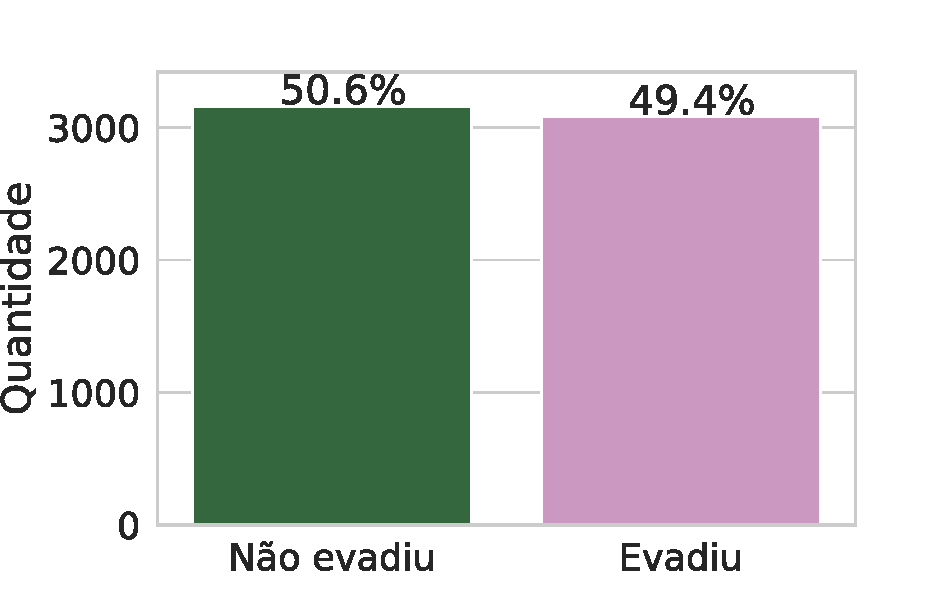
\includegraphics[scale=.29]{img/barplot_pedagogia}}\qquad
  \subcaptionbox{\label{classDistribuitionPedTest}Distribuição para os dados de teste.}{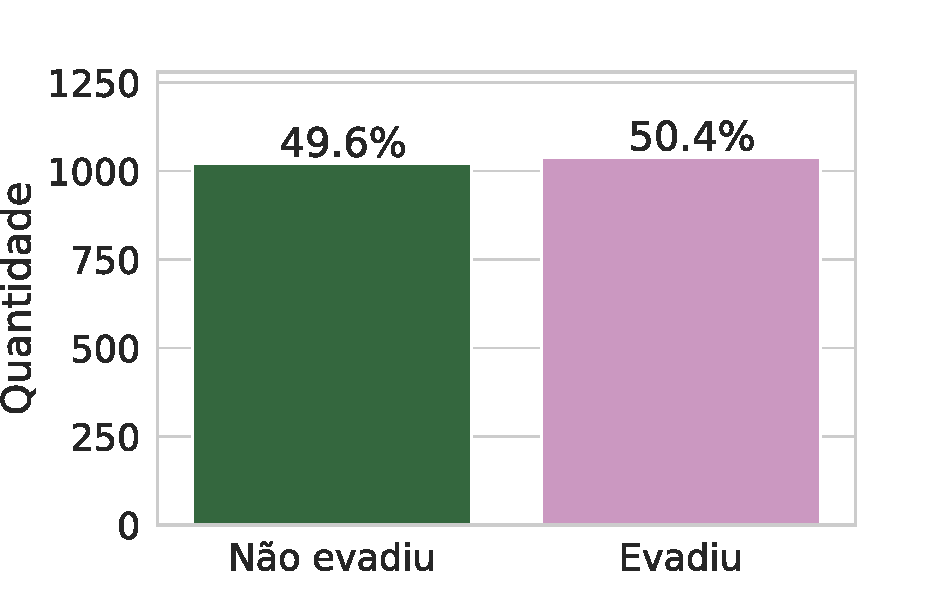
\includegraphics[scale=.29]{img/barplot_pedagogia_testes}}\qquad
  \subcaptionbox{\label{classDistribuitionPedTrain}Distribuição para os dados de treinamento.}{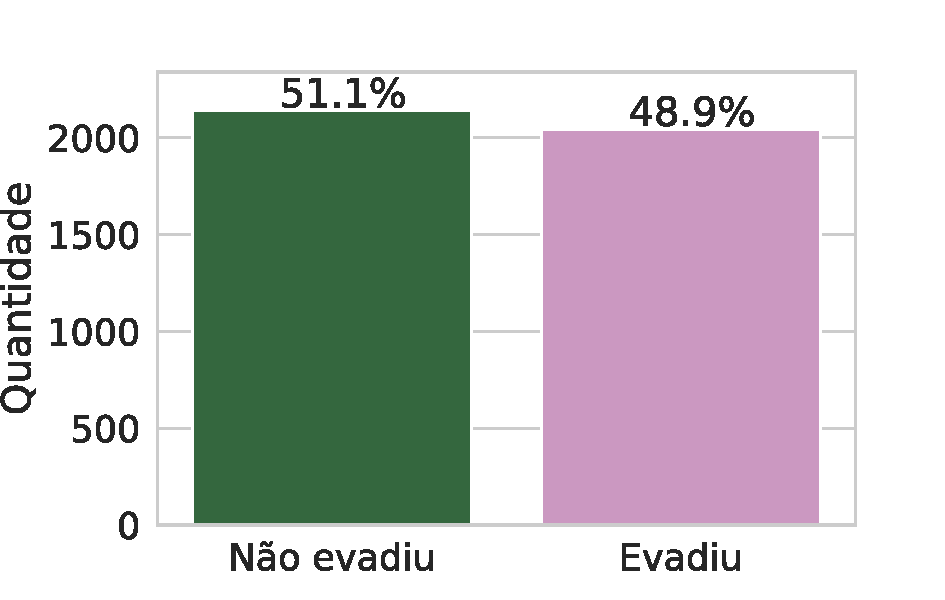
\includegraphics[scale=.29]{img/barplot_pedagogia_treinamento}}
  \vspace{1.5em}
  \Ididthis
\end{figure}

Os dados do curso de Bacharelado em Administração Pública somaram 11685
entradas. Sendo que, $43,9\%$ foram marcados como não evadidos e $56,1\%$ foram
marcados como evadido, como ilustra a Figura \ref{classDistribuitionAdmTotal}. A
proporção das classes após a divisão dos dados em conjunto de testes e conjunto
de treinamento é mostrada nas Figuras \ref{classDistribuitionAdmTest} e
\ref{classDistribuitionAdmTrain}, respectivamente.

\begin{figure}[!htb]
  \centering
  \caption{\label{classDistribuitionAdm} Distribuição de classes para os dados do curso de Bacharelado em Administração Pública.}
  \subcaptionbox{\label{classDistribuitionAdmTotal}Distribuição em todos os dados.}{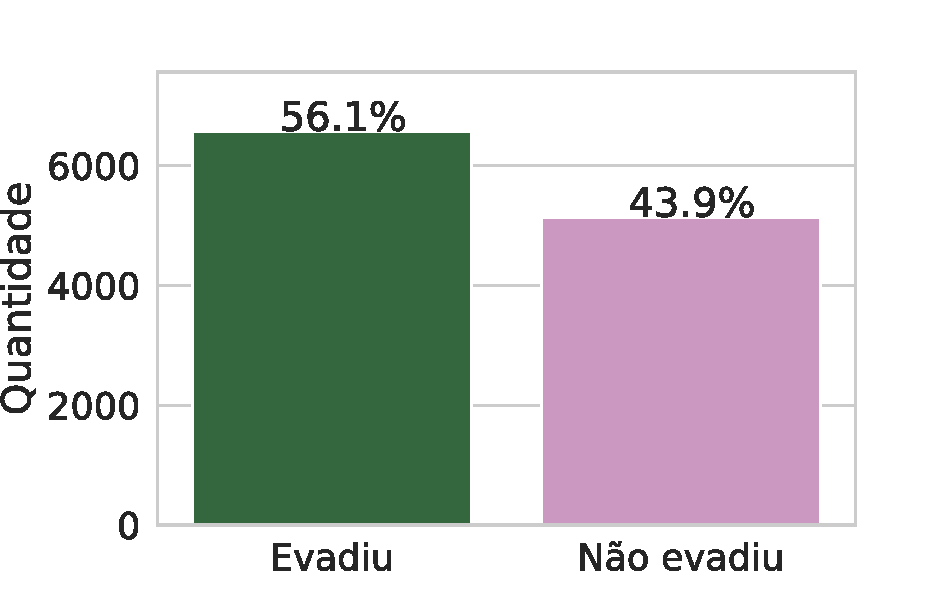
\includegraphics[scale=.29]{img/barplot_adm}}\qquad
  \subcaptionbox{\label{classDistribuitionAdmTest}Distribuição para os dados de teste.}{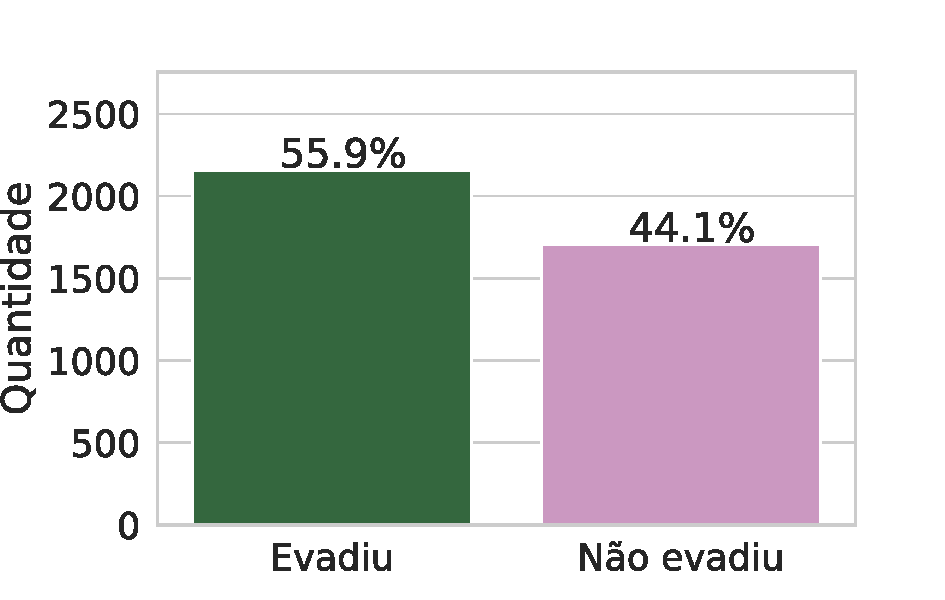
\includegraphics[scale=.29]{img/barplot_adm_testes}}\qquad
  \subcaptionbox{\label{classDistribuitionAdmTrain}Distribuição para os dados de treinamento.}{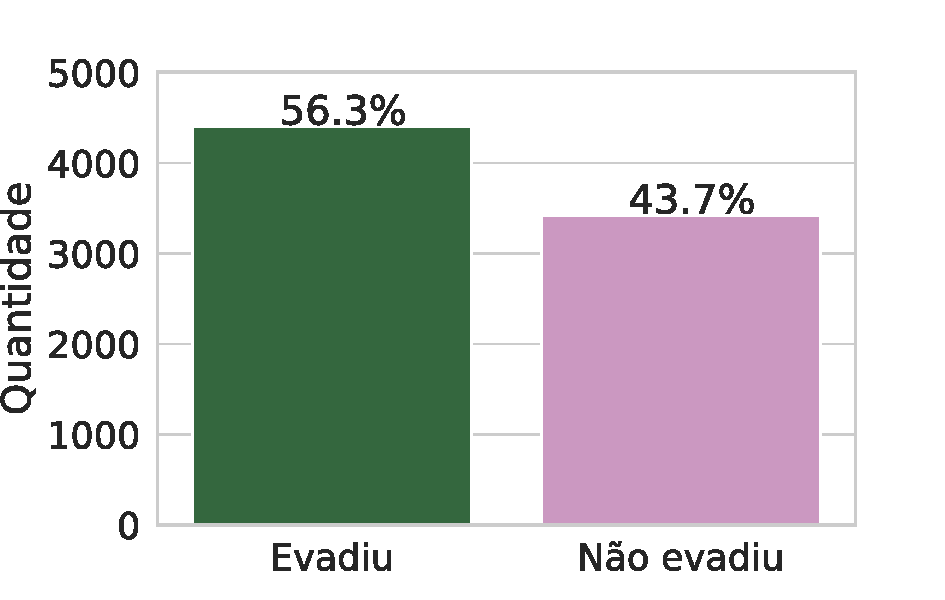
\includegraphics[scale=.29]{img/barplot_adm_treinamento}}
  \vspace{1.5em}
  \Ididthis
\end{figure}

As Tabelas \ref{decribingStatisticsPed} e \ref{decribingStatisticsAdm}
apresentam as estatísticas descritivas das variáveis coletadas no curso de
Licenciatura em Pedagogia e Bacharelado em Administração Pública,
respectivamente.

\begin{table}[!htb]
  \centering
  \caption{Estatísticas descritivas para as variáveis do curso de Licenciatura em Pedagogia}
  \label{decribingStatisticsPed}
  \begin{tabular}{@{}lrrrr@{}}
    \toprule
    \multicolumn{1}{c}{\textbf{Variável}} & \multicolumn{1}{c}{\textbf{Min}} & \multicolumn{1}{c}{\textbf{Média}} & \multicolumn{1}{c}{\textbf{Mediana}} & \multicolumn{1}{c}{\textbf{Max}} \\ \midrule
    VAR01 & 0,00 & 2,19 & 0,00 & 49,00 \\
    VAR02 & 0,00 & 20,45 & 4,00 & 956,00 \\
    VAR03 & 0,00 & 43,46 & 28,00 & 356,00 \\
    VAR04 & 0,00 & 12,89 & 14,00 & 36,00 \\
    VAR05a & 0,00 & 15,91 & 7,00 & 157,00 \\
    VAR05b & 0,00 & 25,77 & 15,00 & 215,00 \\
    VAR05c & 0,00 & 36,70 & 19,00 & 314,00 \\
    VAR06 & 0,00 & 2,89 & 0,00 & 115,00 \\
    VAR07 & 0,00 & 80,87 & 57,00 & 604,00 \\
    VAR08 & 0,00 & 9,82 & 2,00 & 241,00 \\
    VAR09 & 0,00 & 30,39 & 21,00 & 194,00 \\
    VAR10 & 0,00 & 6,79 & 1,00 & 102,00 \\
    VAR11 & 0,00 & 6,78 & 0,00 & 539,00 \\
    VAR12 & 0,00 & 0,29 & 0,00 & 5,00 \\
    VAR12 & 0,00 & 3,97 & 2,67 & 117,17 \\
    VAR14 & 0,00 & 4,71 & 4,00 & 28,00 \\
    VAR15 & 0,00 & 17,74 & 3,00 & 684,00 \\ \bottomrule
  \end{tabular}
\end{table}

\begin{table}[!htb]
  \centering
  \caption{Estatísticas descritivas para as variáveis do curso de Bacharelado em Administração Pública}
  \label{decribingStatisticsAdm}
  \begin{tabular}{@{}lrrrr@{}}
    \toprule
    \textbf{Variável} & \multicolumn{1}{l}{\textbf{Min}} & \multicolumn{1}{l}{\textbf{Média}} & \multicolumn{1}{l}{\textbf{Mediana}} & \multicolumn{1}{l}{\textbf{Max}} \\ \midrule
    VAR01 & 0,00 & 1,42 & 0,00 & 59,00 \\
    VAR02 & 0,00 & 21,66 & 2,00 & 1797,00 \\
    VAR03 & 0,00 & 61,59 & 43,00 & 1114,00 \\
    VAR04 & 0,00 & 17,70 & 17,00 & 81,00 \\
    VAR05a & 0,00 & 20,60 & 7,00 & 402,00 \\
    VAR05b & 0,00 & 27,46 & 14,00 & 342,00 \\
    VAR05c & 0,00 & 29,96 & 15,00 & 272,00 \\
    VAR06 & 0,00 & 1,09 & 0,00 & 96,00 \\
    VAR07 & 0,00 & 80,40 & 50,00 & 1000,00 \\
    VAR08 & 0,00 & 13,22 & 1,00 & 346,00 \\
    VAR09 & 0,00 & 48,89 & 32,00 & 471,00 \\
    VAR10 & 0,00 & 5,22 & 0,00 & 626,00 \\
    VAR11 & 0,00 & 5,08 & 0,00 & 1598,00 \\
    VAR12 & 0,00 & 0,13 & 0,00 & 6,00 \\
    VAR12 & 0,00 & 2,65 & 1,67 & 55,10 \\
    VAR14 & 0,00 & 4,66 & 5,00 & 20,00 \\
    VAR15 & 0,00 & 9,55 & 0,00 & 533,00 \\ \bottomrule
  \end{tabular}
\end{table}

Sabendo-se dessas informações, principiaram-se os experimentos com os algoritmos
de classificação. Destes, o primeiro foi o KNN. Iniciou-se pela escolha do
parâmetro \(k\), a quantidade de vizinhos. Para tal, foram testados valores
entre \(3\) e \(201\), mantendo-se sempre uma quantidade impar de vizinhos. Esse
experimento foi repetido, porém, com os dados normalizados, na tentativa de
remover a influência da diferença de escalas entre as variáveis. Nas Figuras
\ref{knnKResultsPed} e \ref{knnKResultsAdm} podemos ver os gráficos resultantes
desses experimentos.

\begin{figure}[!htb]
  \centering
  \caption{\label{knnKResultsPed} Gráficos de valores de acurácia para valores de K, com K variando entre \(3\) e \(201\) com incremento de \(2\) para o curso de Licenciatura em Pedagogia.}
  \subcaptionbox{\label{knnKResultsPedA}Dados não normalizados.}{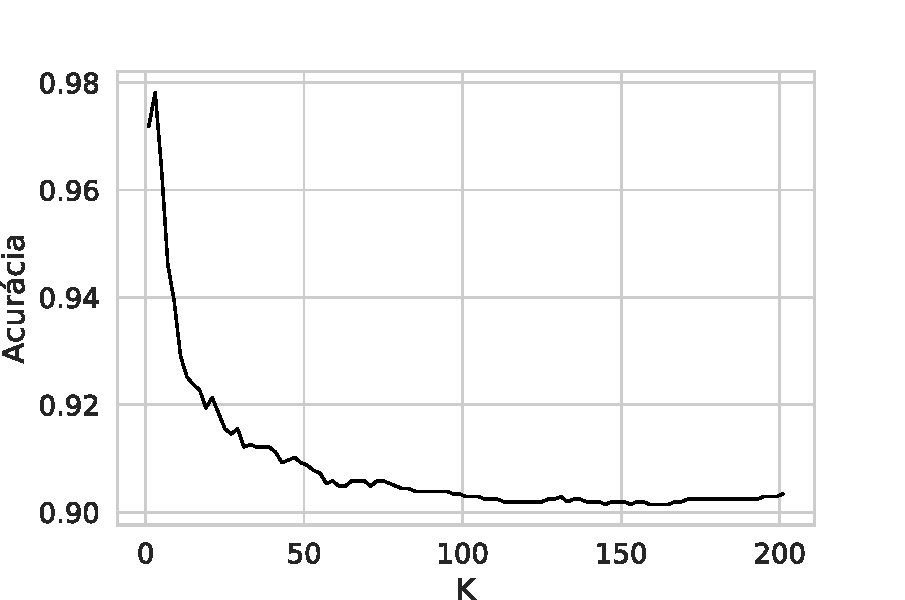
\includegraphics[scale=.45]{img/knn_neigh_ped}}\qquad
  \subcaptionbox{Dados normalizados.}{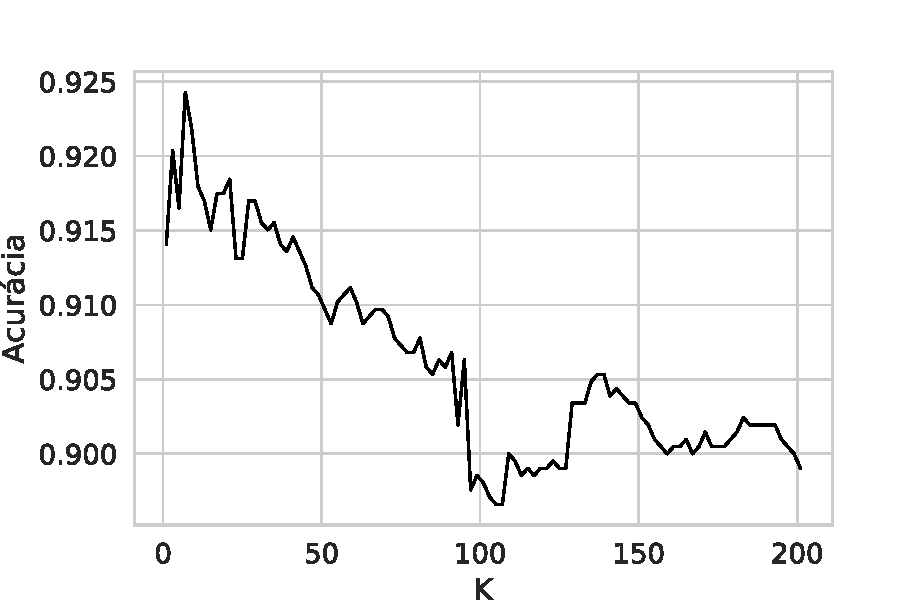
\includegraphics[scale=.45]{img/knn_neigh_norm_ped}}
  \vspace{1.5em}
  \Ididthis
\end{figure}

\begin{figure}[!htb]
  \centering
  \caption{\label{knnKResultsAdm} Gráficos de valores de acurácia para valores de K, com K variando entre \(3\) e \(201\) com incremento de \(2\) para o cuso de Bacharelado em Administração Pública.}
  \subcaptionbox{\label{knnKResultsAdmA}Dados não normalizados.}{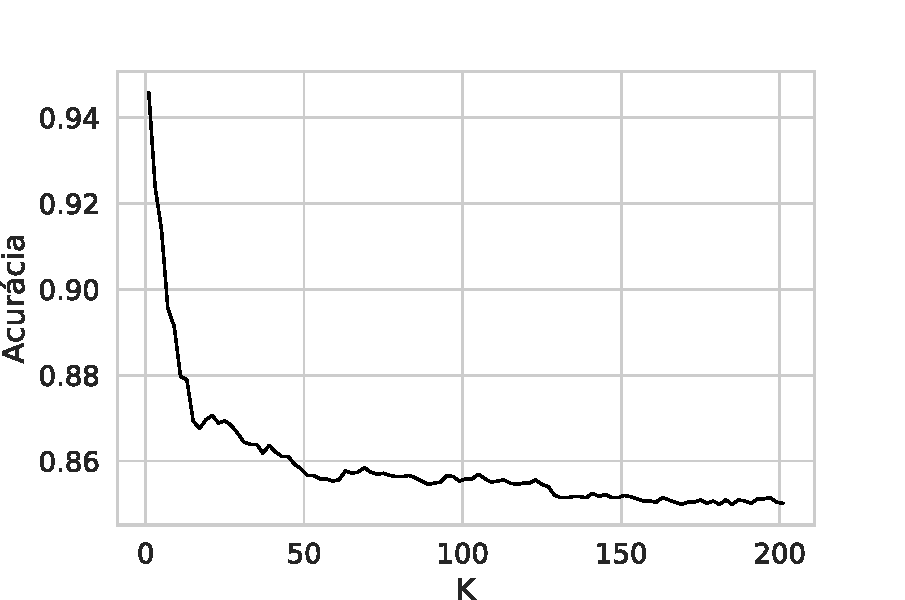
\includegraphics[scale=.45]{img/knn_neigh_adm}}\qquad
  \subcaptionbox{Dados normalizados.}{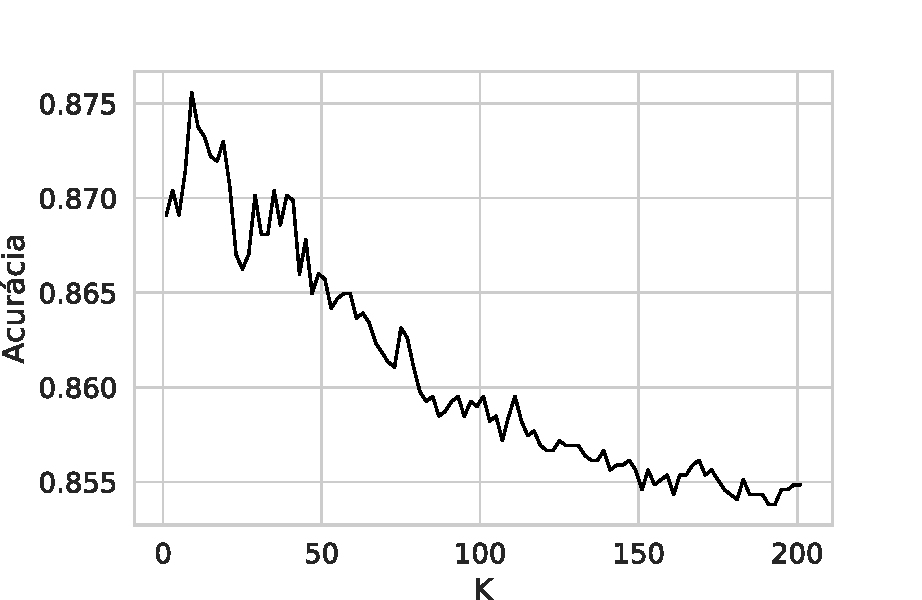
\includegraphics[scale=.45]{img/knn_neigh_norm_adm}}
  \vspace{1.5em}
  \Ididthis
\end{figure}

A acurácia do algoritmo foi escolhida como métrica nesses experimentos por ser
uma métrica clássica e utilizada como padrão na biblioteca \textit{Scikt-learn}.

A partir da análise dos gráficos das Figuras \ref{knnKResultsPedA} e
\ref{knnKResultsAdmA}, foi escolhido o valor \(3\) para o parâmetro \(k\) na
aplicação do KNN sobre os dados do curso de Licenciatura em Pedagogia e o valor
\(1\) para o curso de Bacharelado em Administração Pública.

Os algoritmos Árvore de Decisão e Regressão Logística não possuem parâmetros,
portanto, não tiveram que passar pelo mesmo processo que o KNN.

Cada algoritmo foi treinado com os conjuntos de treinamento e testado com o
conjunto de testes. Após, foram calculadas as matrizes de confusão, que estão
ilustradas na Figura \ref{confusionMatrixResult}.

\begin{figure}[!htb]
  \centering
  \caption{\label{confusionMatrixResult} Matrizes de confusão.}
  \subcaptionbox{KNN Administração.}{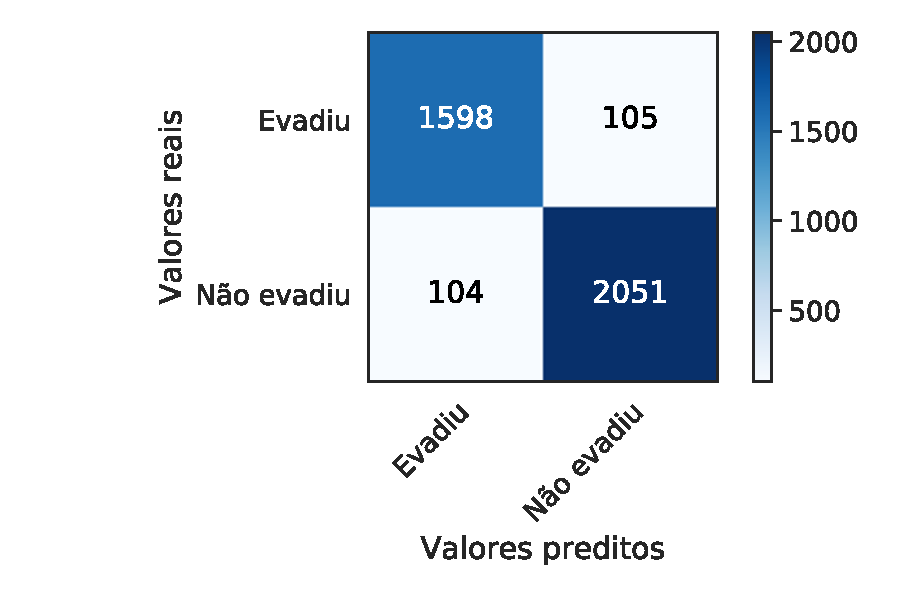
\includegraphics[scale=.40]{img/cm_knn_adm}}\qquad
  \subcaptionbox{LR Administração.}{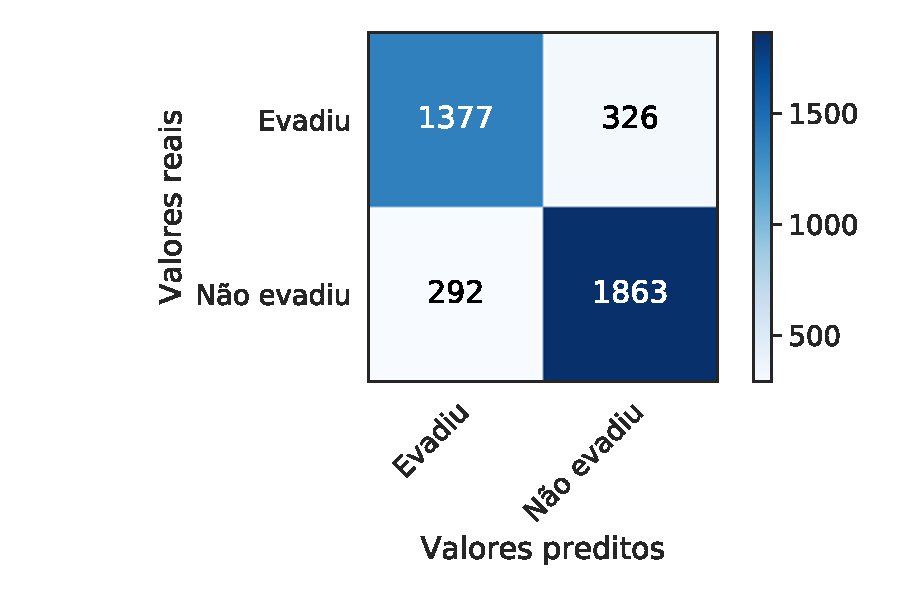
\includegraphics[scale=.40]{img/cm_rl_adm}}\qquad
  \subcaptionbox{Árvore de Decisçao Administração.}{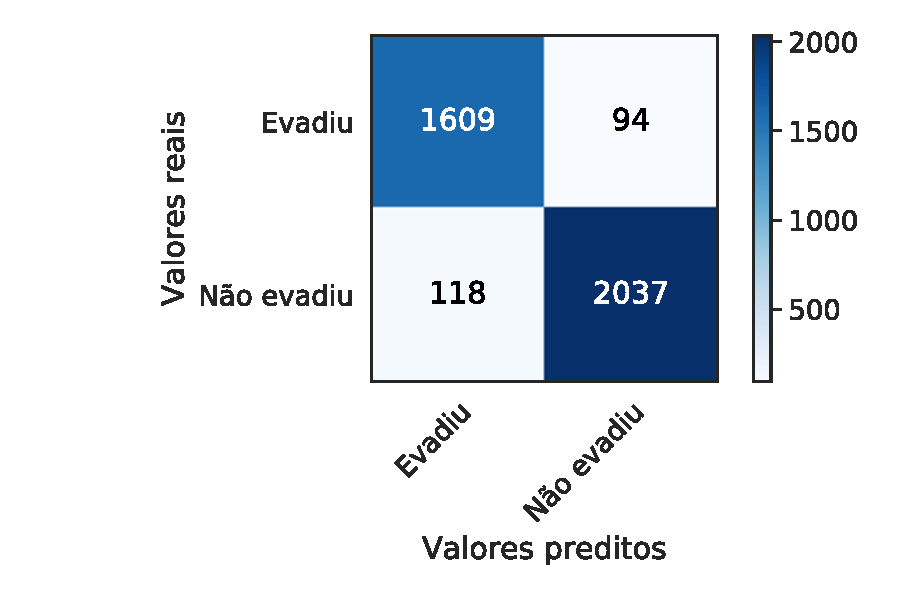
\includegraphics[scale=.40]{img/cm_tree_adm}}
  \subcaptionbox{KNN Pedagogia.}{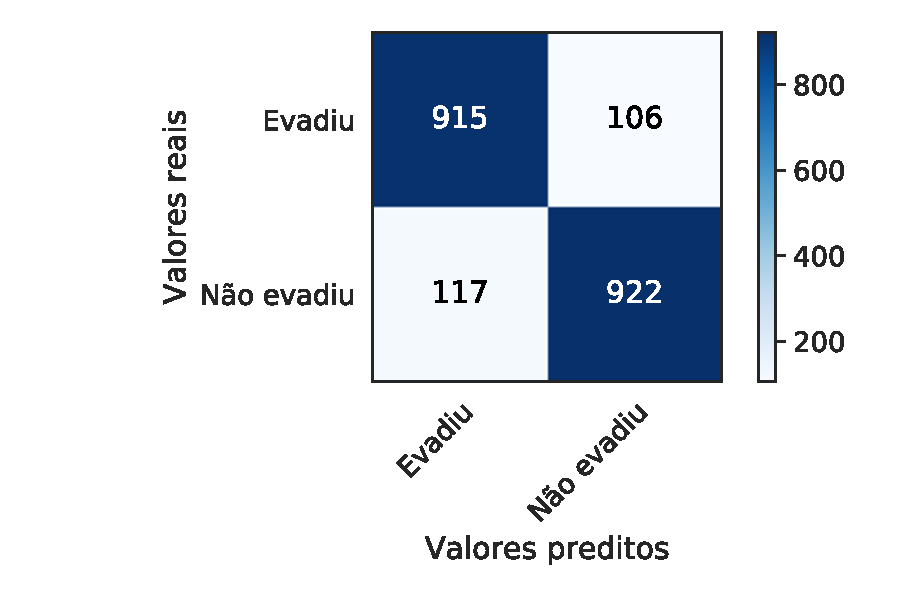
\includegraphics[scale=.40]{img/cm_knn_ped}}\qquad
  \subcaptionbox{LR Pedagogia.}{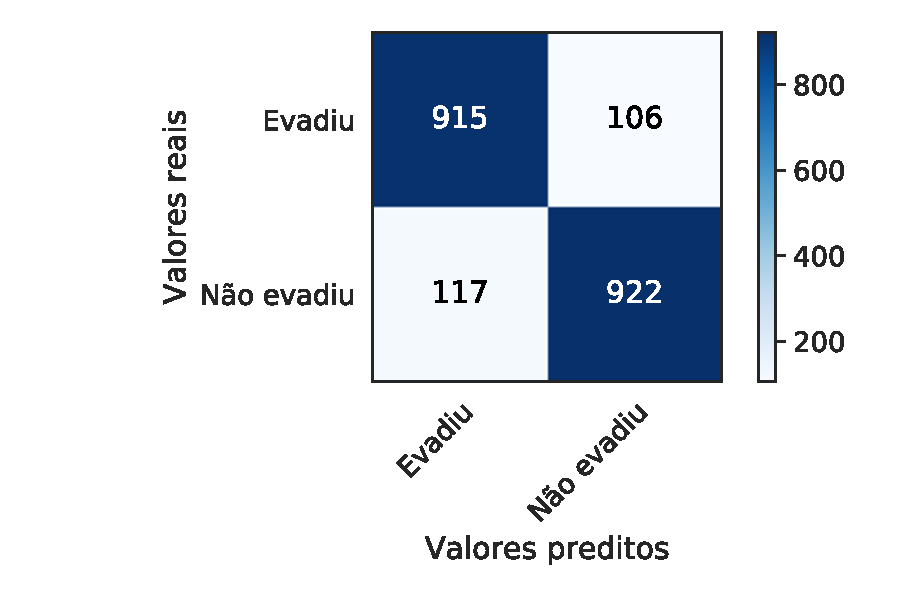
\includegraphics[scale=.40]{img/cm_rl_ped}}\qquad
  \subcaptionbox{Árvore de Decisçao Pedagogia.}{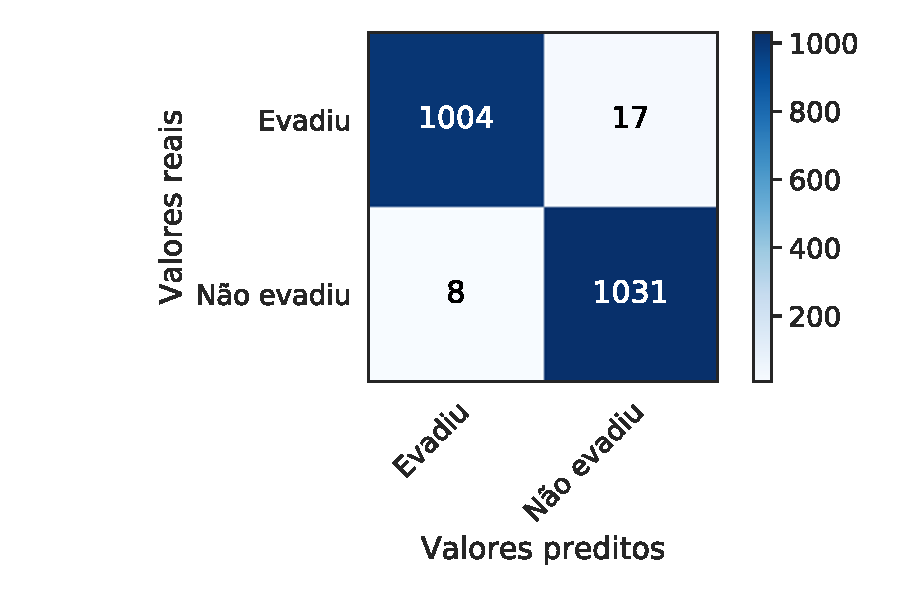
\includegraphics[scale=.40]{img/cm_tree_ped}}
  \vspace{1.5em}
  \Ididthis
\end{figure}

As matrizes de confusão serviram como base para o cálculo das métricas dos
algoritmos de classificação, as Tabelas \ref{metricsPed} e \ref{metricsAdm}
apresentam os resultados para cada algoritmo.

\begin{table}[!htb]
  \centering
  \caption{Métricas dos algoritmos aplicados no curso de Licenciatura em Pedagogia}
  \label{metricsPed}
  \resizebox{\textwidth}{!}{%
  \begin{tabular}{@{}lrrrrrr@{}}
    \toprule
    \multicolumn{1}{c}{\textbf{Algoritmo}} & \multicolumn{1}{c}{\textbf{Acurácia}} & \multicolumn{1}{c}{\textbf{Precisão}} & \multicolumn{1}{c}{\textbf{Sensibilidade}} & \multicolumn{1}{c}{\textbf{Especificidade}} & \multicolumn{1}{c}{\textbf{TFP}} & \multicolumn{1}{c}{\textbf{TFN}} \\ \midrule
    KNN & 0,9782 & 0,9770 & 0,9798 & 0,9383 & 0,0235 & 0.0202 \\
    Árvore de Decisão & 0,9879 & 0,9838 & 0,9923 & 0,9833 & 0,0167 & 0,0077 \\
    Regressão Logística & 0,8917 & 0,8969 & 0,8874 & 0,8962 & 0,1038 & 0,1126 \\ \bottomrule
  \end{tabular}%
  }
  \Ididthis
\end{table}

\begin{table}[!htb]
  \centering
  \caption{Métricas dos algoritmos aplicados no curso de Bacharelado em Administração Pública}
  \label{metricsAdm}
    \resizebox{\textwidth}{!}{%
    \begin{tabular}{@{}lrrrrrr@{}}
    \toprule
    \multicolumn{1}{c}{\textbf{Algoritmo}} & \multicolumn{1}{c}{\textbf{Acurácia}} & \multicolumn{1}{c}{\textbf{Precisão}} & \multicolumn{1}{c}{\textbf{Sensibilidade}} & \multicolumn{1}{c}{\textbf{Especificidade}} & \multicolumn{1}{c}{\textbf{TFP}} & \multicolumn{1}{c}{\textbf{TFN}} \\ \midrule
    KNN & 0,9458 & 0,9513 & 0,9517 & 0,9383 & 0,0617 & 0,0483 \\
    Árvore de Decisão & 0,9419 & 0,9526 & 0,9429 & 0,9407 & 0,0593 & 0,0571 \\
    Regressão Logística & 0,8398 & 0,8511 & 0,8645 & 0,8086 & 0,1914 & 0,1355 \\ \bottomrule
  \end{tabular}%
  }
  \Ididthis
\end{table}

Para o algoritmo de Árvore de Decisão foram geradas as visualizações das árvores
para os \(3\) primeiros níveis, que estão ilustrados nas Figuras \ref{treePed} e
\ref{treeAdm}. No nó raiz dessas árvores fica a variável com maior importância
para o algoritmo.

\begin{figure}[!htb]
  \centering
  \caption{\label{treePed} Árvore de Decisão gerada a partir dos dados do curso de Licenciatura em Pedagogia.}
  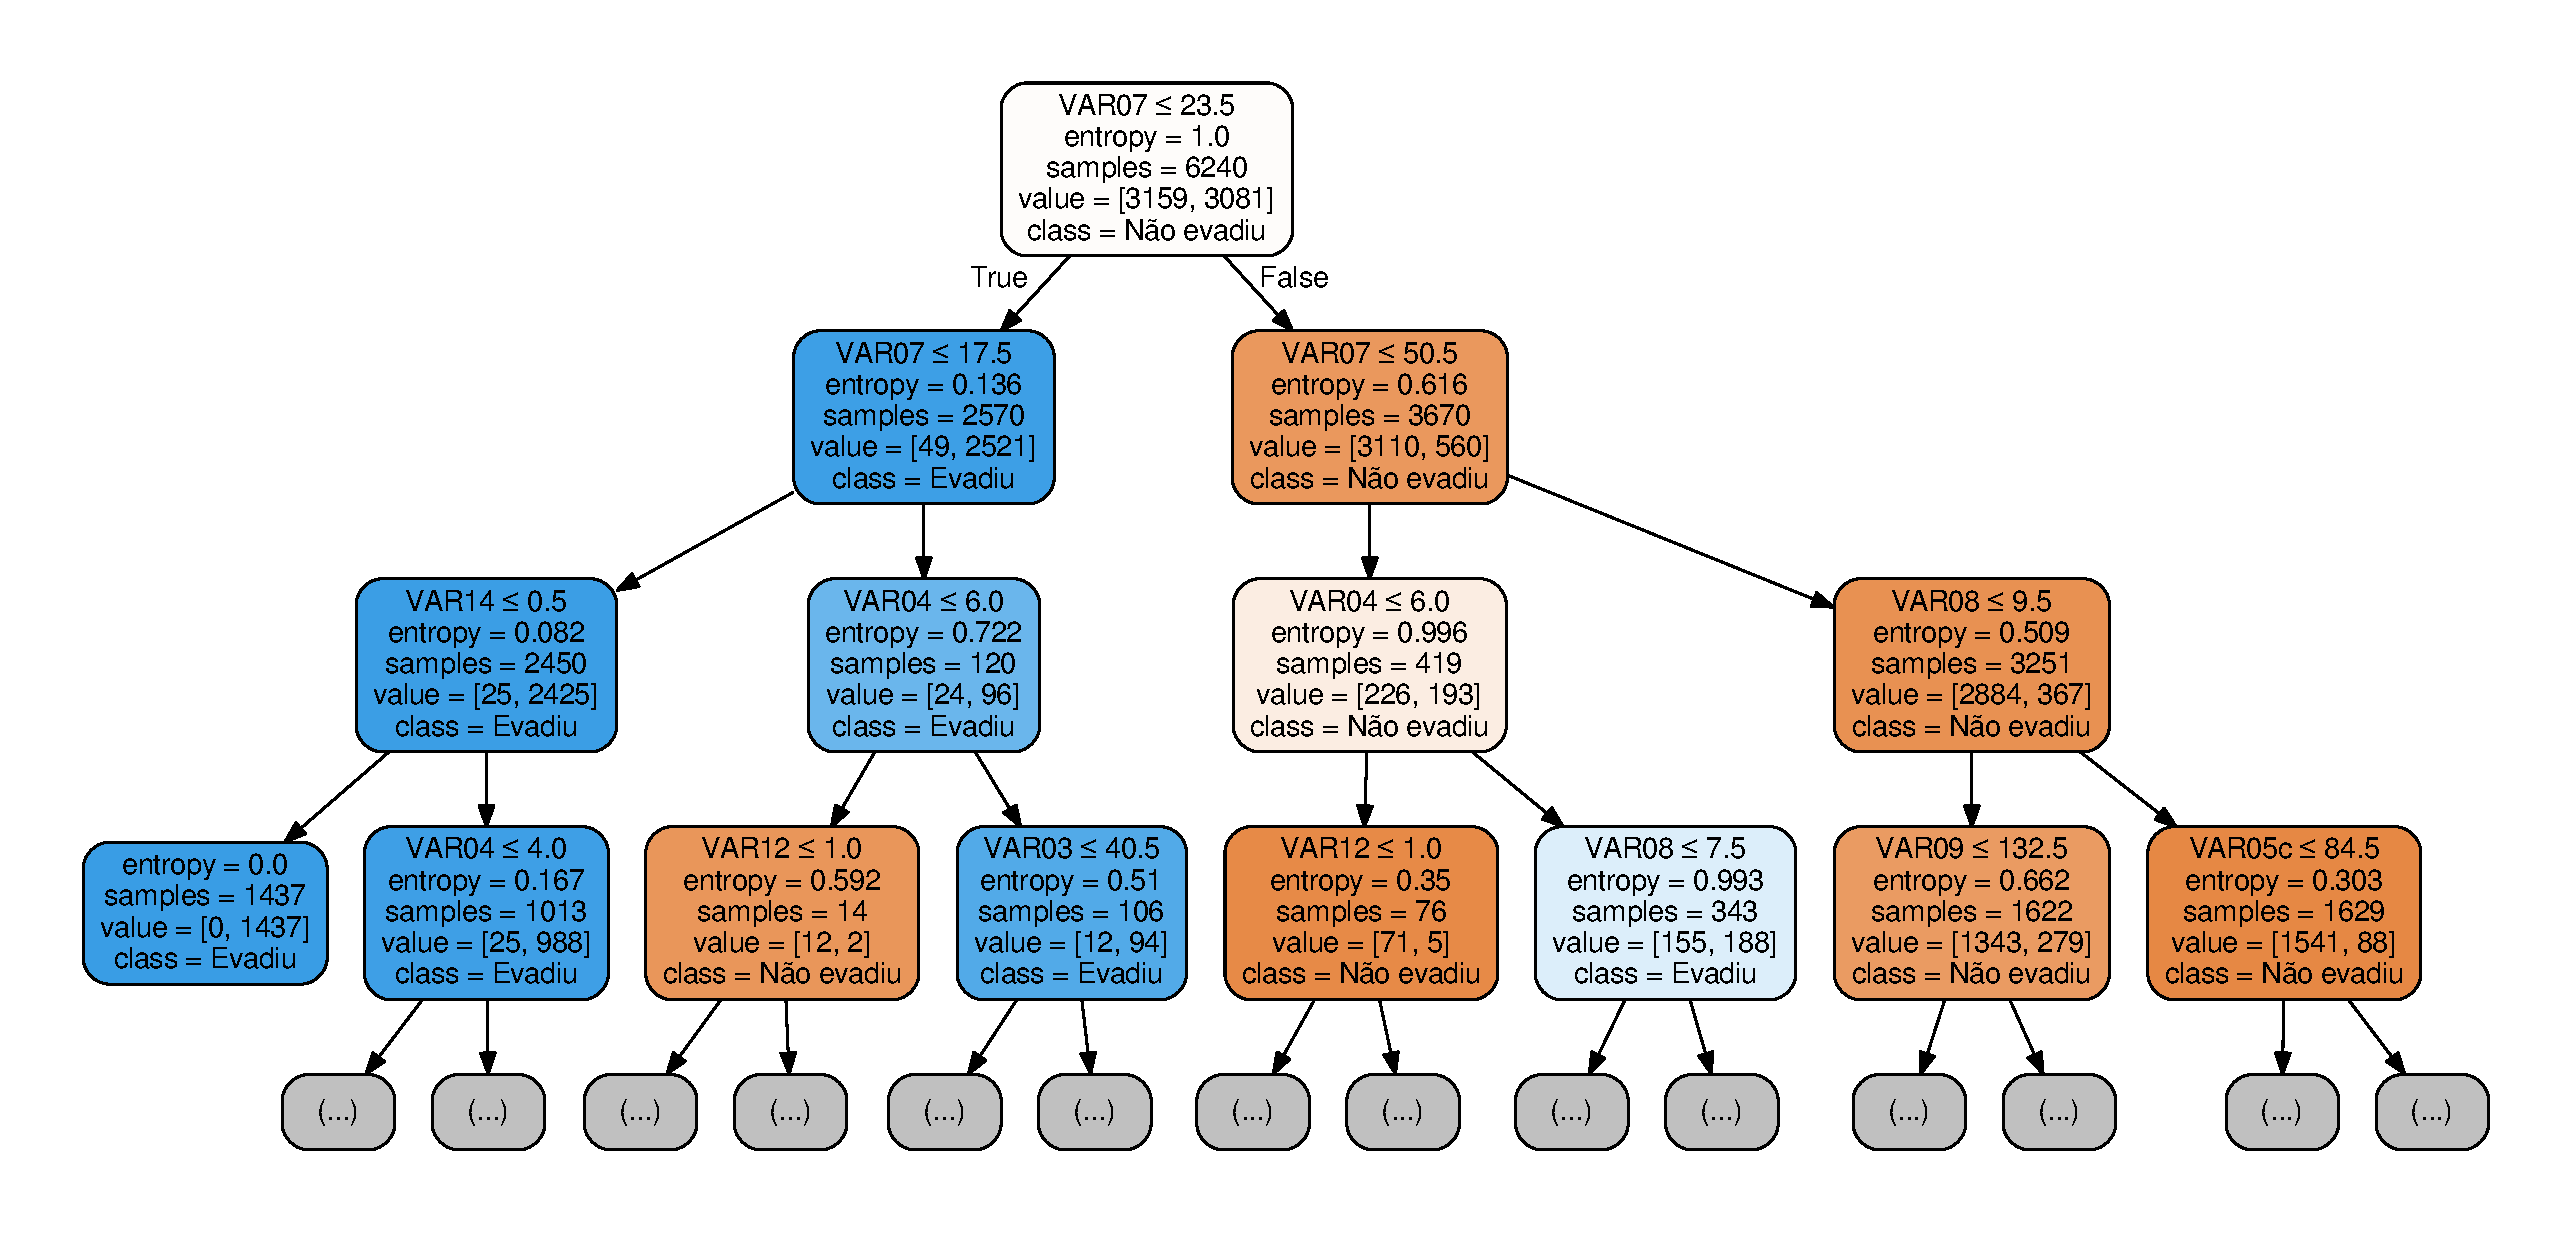
\includegraphics[angle=-90,scale=.50]{img/ped_tree}
  \Ididthis
\end{figure}

\begin{figure}[!htb]
  \centering
  \caption{\label{treeAdm} Árvore de Decisão gerada a partir dos dados do curso de Bacharelado em Administração Pública.}
  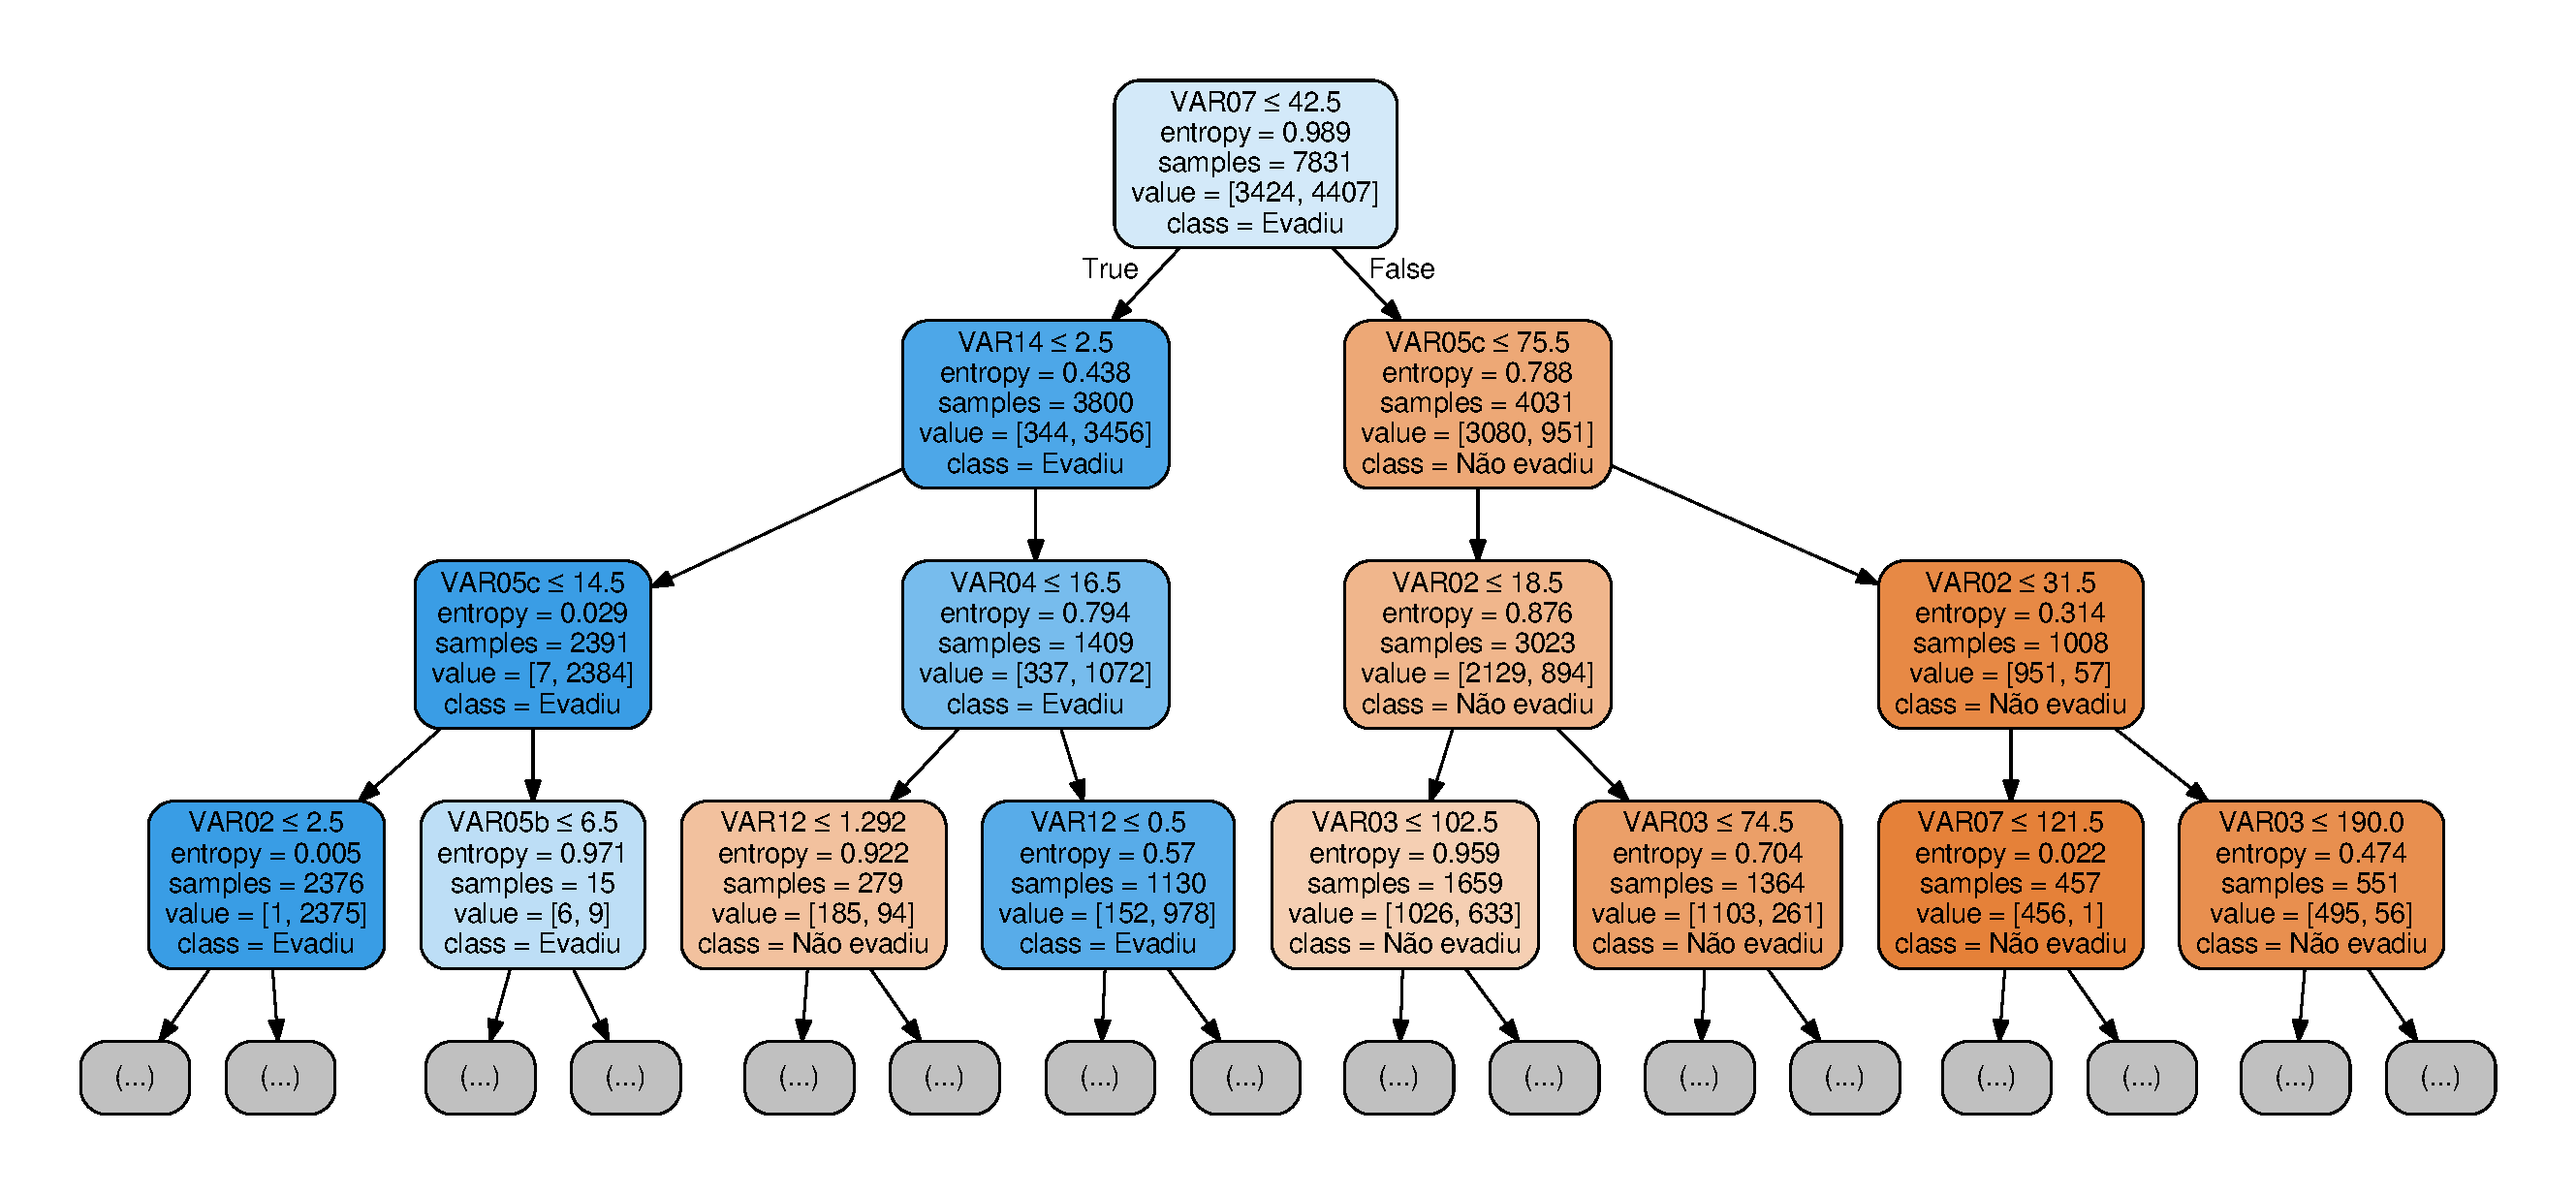
\includegraphics[angle=-90,scale=.50]{img/adm_tree}
  \Ididthis
\end{figure}

Notou-se que a variável \textit{VAR07} (Quantidade de acessos do aluno ao
ambiente no semestre) apareceu como a mais relevante. Porém, como todas as
outras variáveis só são contabilizadas depois que o aluno acessa o ambiente,
essa variável se torna bastante enviesada. Devido a isso, a etapa de mineração
foi executada novamente com a exclusão da mesma.

Para o algoritmo KNN, o valor de \(k\) foi ajustado para os dados sem a variável
\textit{VAR07}. As Figuras \ref{knnKResultsPedNoVar7} e
\ref{knnResultsAdmNoVar7} ilustram os gráficos utilizados para a escolha do
parâmetro \(k\).

\begin{figure}[!htb]
  \centering
  \caption{\label{knnKResultsPedNoVar7} Gráficos de valores de acurácia para valores de K, com K variando entre \(3\) e \(201\) com incremento de \(2\) para o curso de Licenciatura em Pedagogia após a exclusão da variável \textit{VAR07}.}
  \subcaptionbox{\label{knnKResultsPedANoVar7A}Dados não normalizados.}{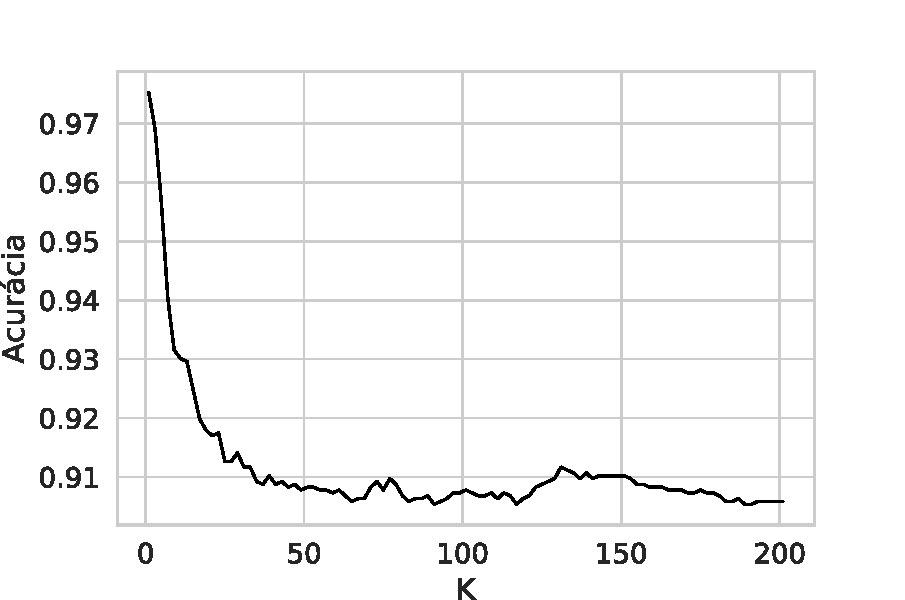
\includegraphics[scale=.45]{img/knn_neigh_ped_no_var07}}\qquad
  \subcaptionbox{Dados normalizados.}{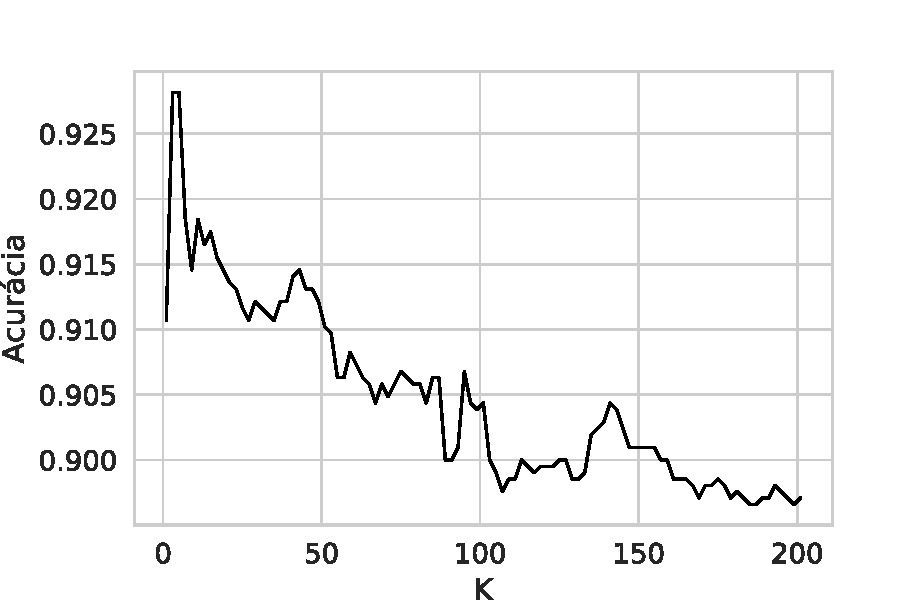
\includegraphics[scale=.45]{img/knn_neigh_norm_ped_no_var07}}
  \vspace{1.5em}
  \Ididthis
\end{figure}

\begin{figure}[!htb]
  \centering
  \caption{\label{knnResultsAdmNoVar7} Gráficos de valores de acurácia para valores de K, com K variando entre \(3\) e \(201\) com incremento de \(2\) para o cuso de Bacharelado em Administração Pública após a exclusão da variável \textit{VAR07}.}
  \subcaptionbox{\label{knnKResultsAdmANoVar7A}Dados não normalizados.}{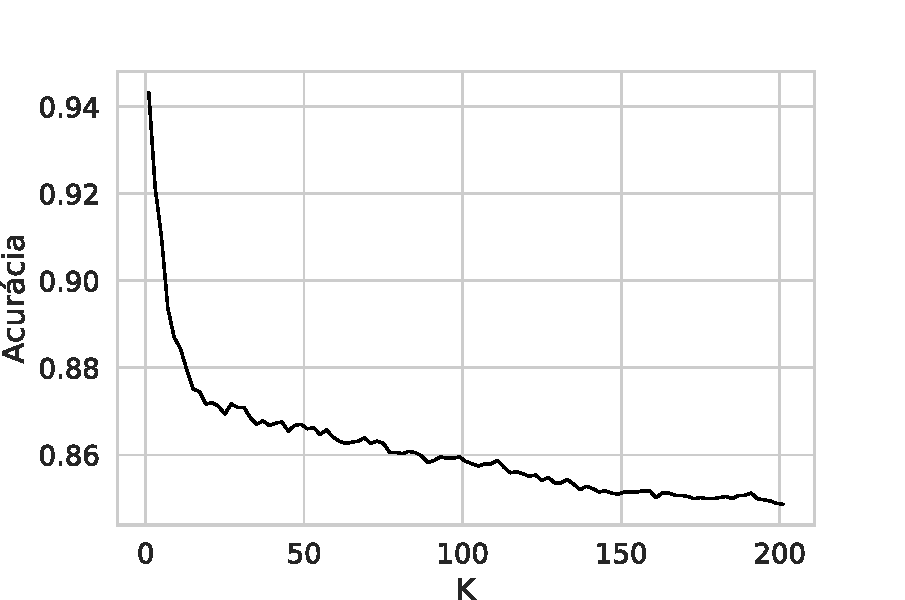
\includegraphics[scale=.45]{img/knn_neigh_adm_no_var07}}\qquad
  \subcaptionbox{Dados normalizados.}{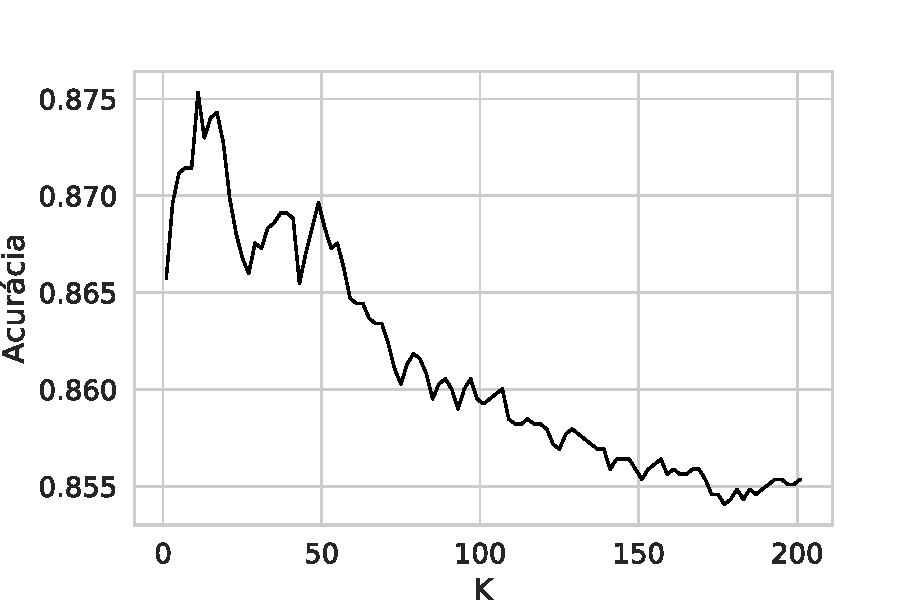
\includegraphics[scale=.45]{img/knn_neigh_norm_adm_no_var07}}
  \vspace{1.5em}
  \Ididthis
\end{figure}

Após análise dos gráficos contidos nas Figuras \ref{knnKResultsPedANoVar7A} e
\ref{knnKResultsAdmANoVar7A}, optou-se para valores de \(k = 1\) e os dados não
normalizados em ambas as bases.

Em seguida, foram geradas novas matrizes de confusão que estão ilustradas na Figura \ref{newConfusionMatrixResult}.

\begin{figure}[!htb]
  \centering
  \caption{\label{newConfusionMatrixResult} Matrizes de confusão após a exclusão da \textit{VAR07}.}
  \subcaptionbox{KNN Administração.}{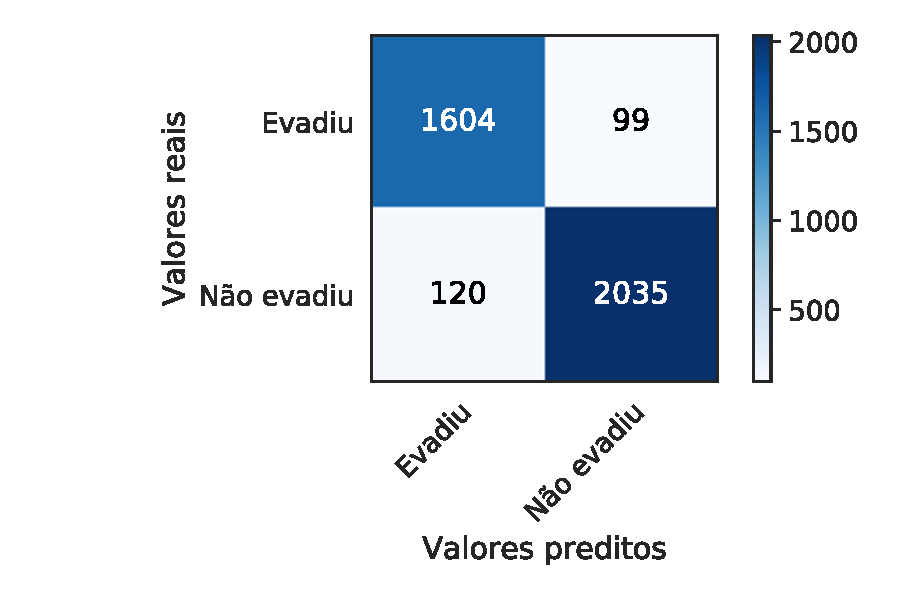
\includegraphics[scale=.40]{img/cm_knn_adm_no_var07}}\qquad
  \subcaptionbox{LR Administração.}{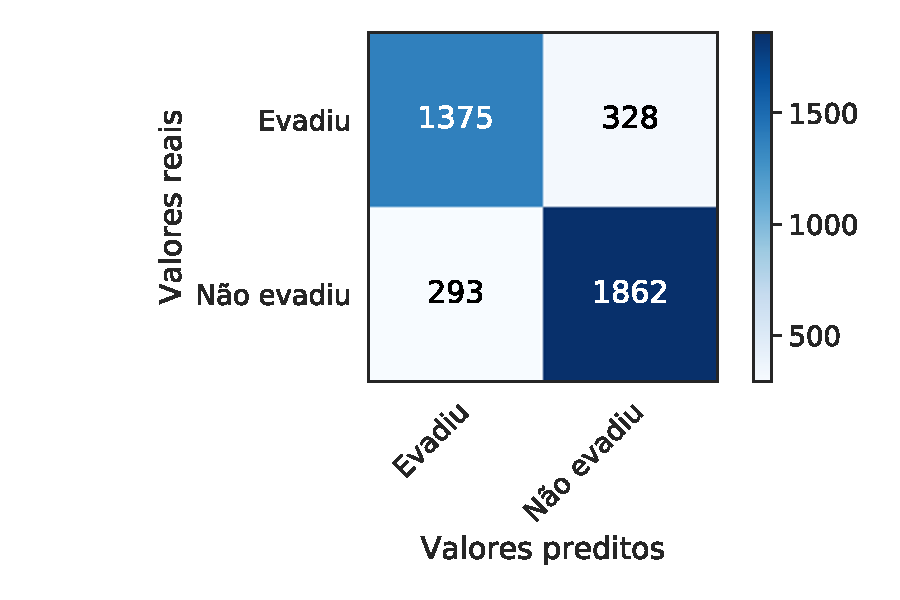
\includegraphics[scale=.40]{img/cm_rl_adm_no_var07}}\qquad
  \subcaptionbox{Árvore de Decisçao Administração.}{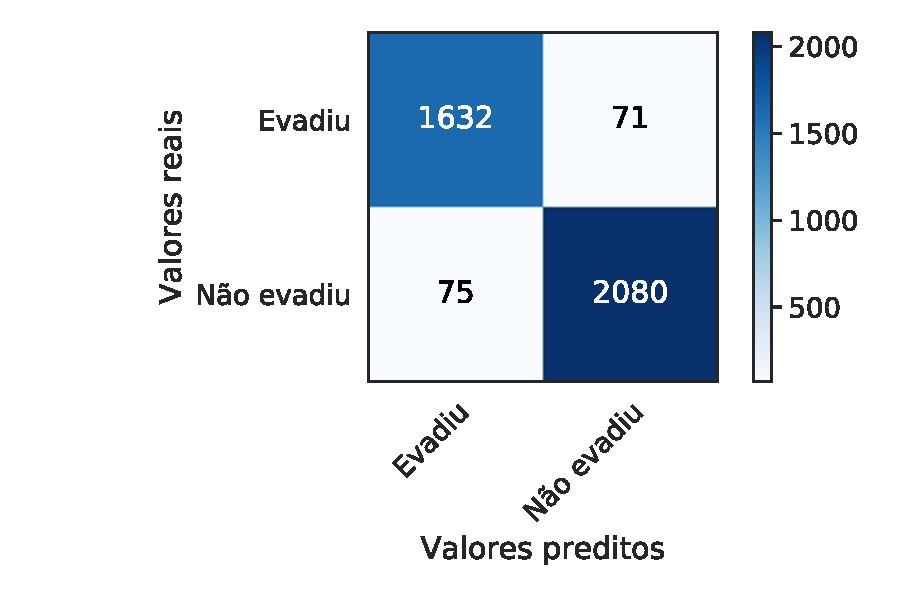
\includegraphics[scale=.40]{img/cm_tree_adm_no_var07}}
  \subcaptionbox{KNN Pedagogia.}{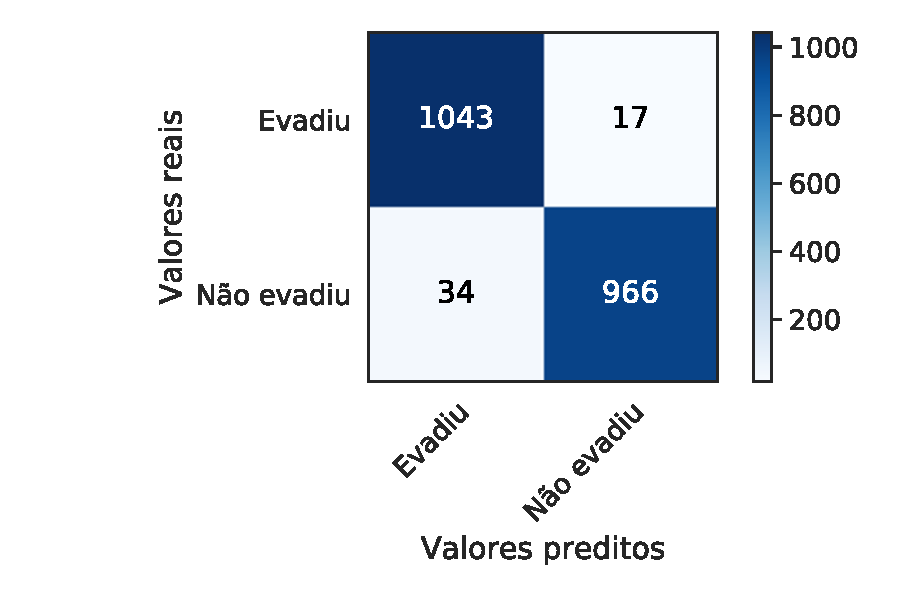
\includegraphics[scale=.40]{img/cm_knn_ped_no_var07}}\qquad
  \subcaptionbox{LR Pedagogia.}{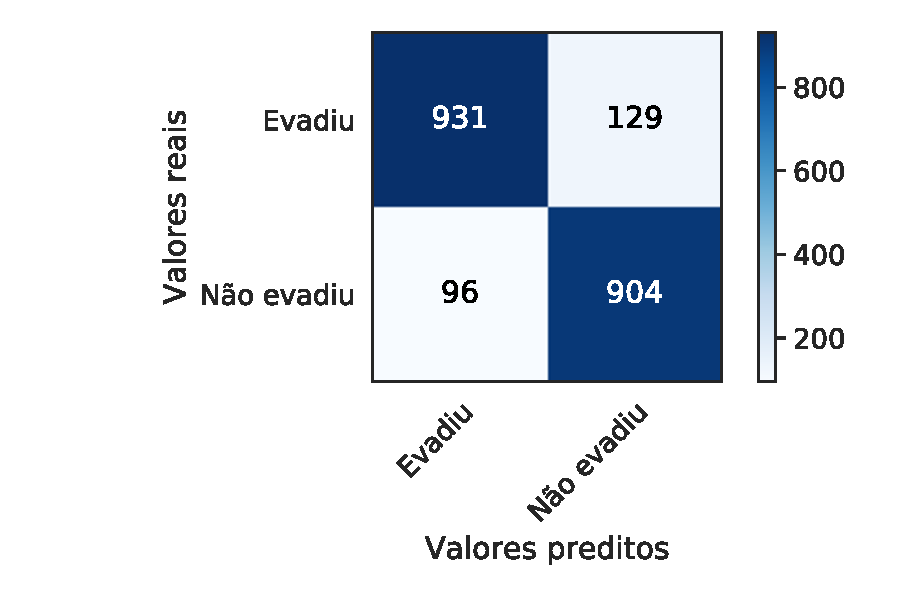
\includegraphics[scale=.40]{img/cm_rl_ped_no_var07}}\qquad
  \subcaptionbox{Árvore de Decisçao Pedagogia.}{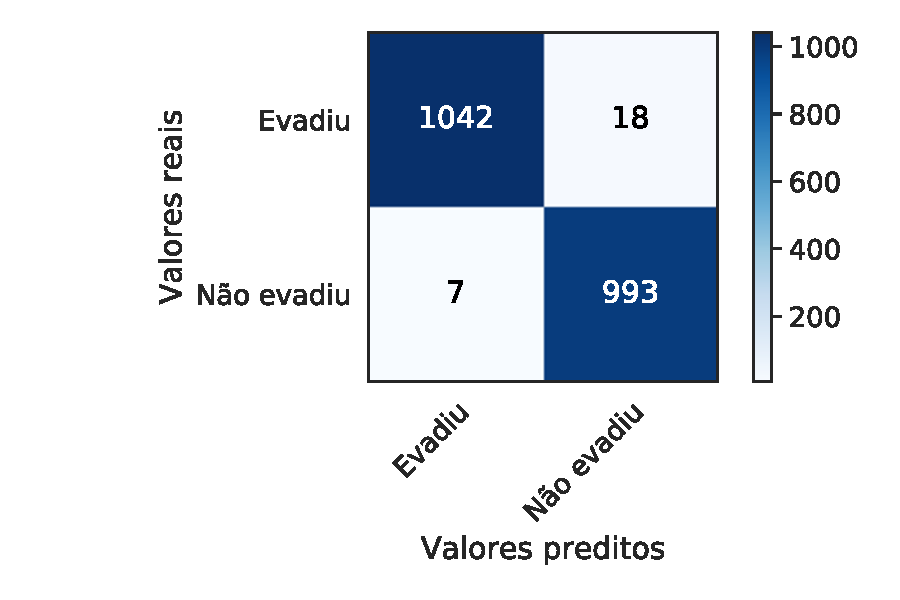
\includegraphics[scale=.40]{img/cm_tree_ped_no_var07}}
  \vspace{1.5em}
  \Ididthis
\end{figure}

Também foi realizada a análise da árvore de decisão gerada depois da remoção da
variável \textit{VAR07}. A representação gráfica das árvores para o curso de
Licenciatura em Pedagogia e Bacharelado em Administração Pública estão
ilustradas nas Figuras \ref{treePedNoVar07} e \ref{treeAdmNoVar07},
respectivamente.

\begin{figure}[!htb]
  \centering
  \caption{\label{treePedNoVar07} Árvore de Decisão gerada a partir dos dados do curso de Licenciatura em Pedagogia.}
  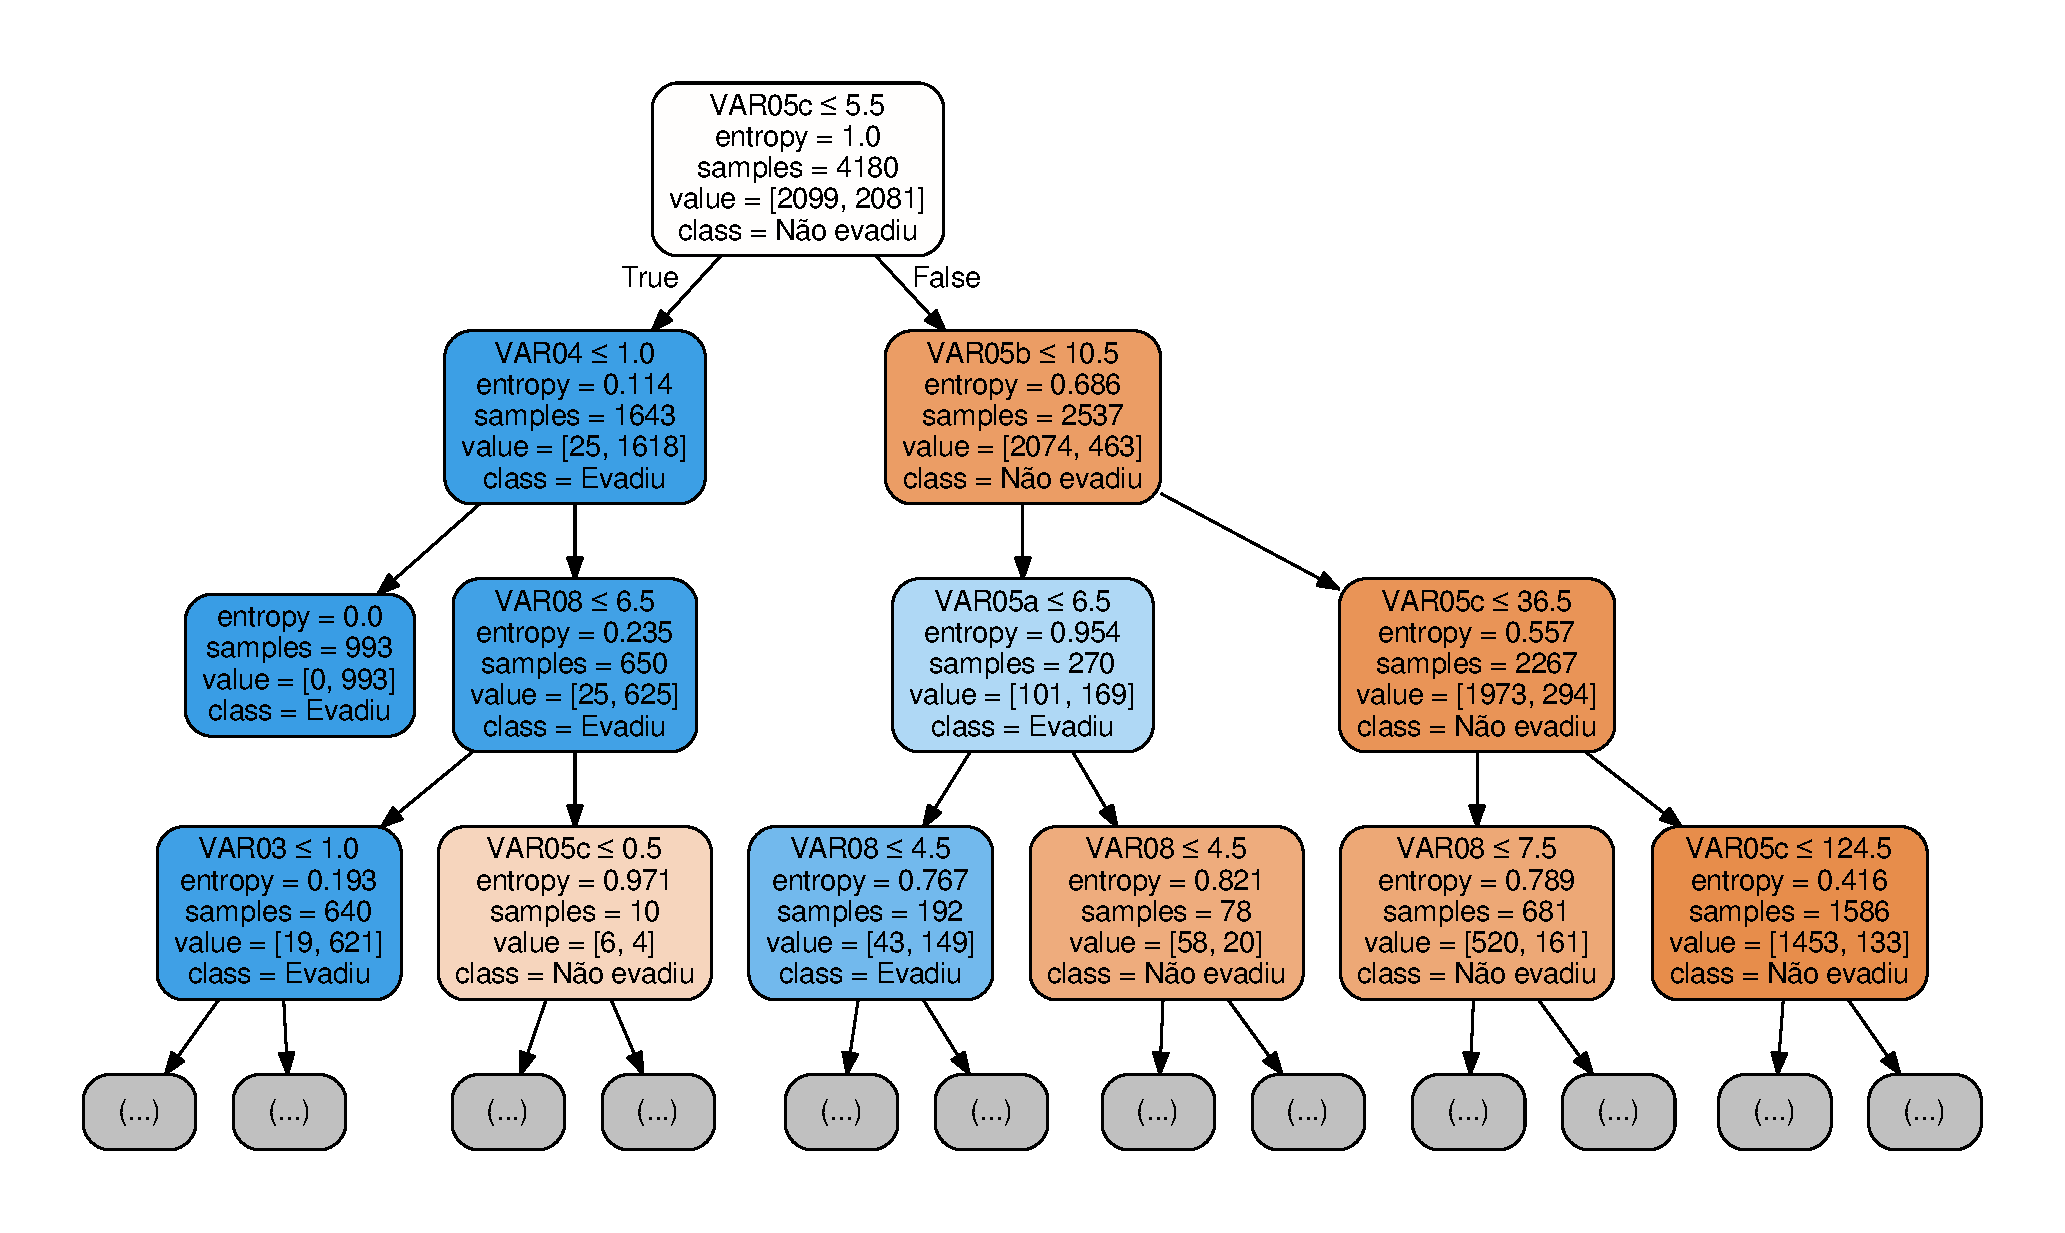
\includegraphics[angle=-90,scale=.50]{img/ped_tree_no_var07}
  \Ididthis
\end{figure}

\begin{figure}[!htb]
  \centering
  \caption{\label{treeAdmNoVar07} Árvore de Decisão gerada a partir dos dados do curso de Bacharelado em Administração Pública.}
  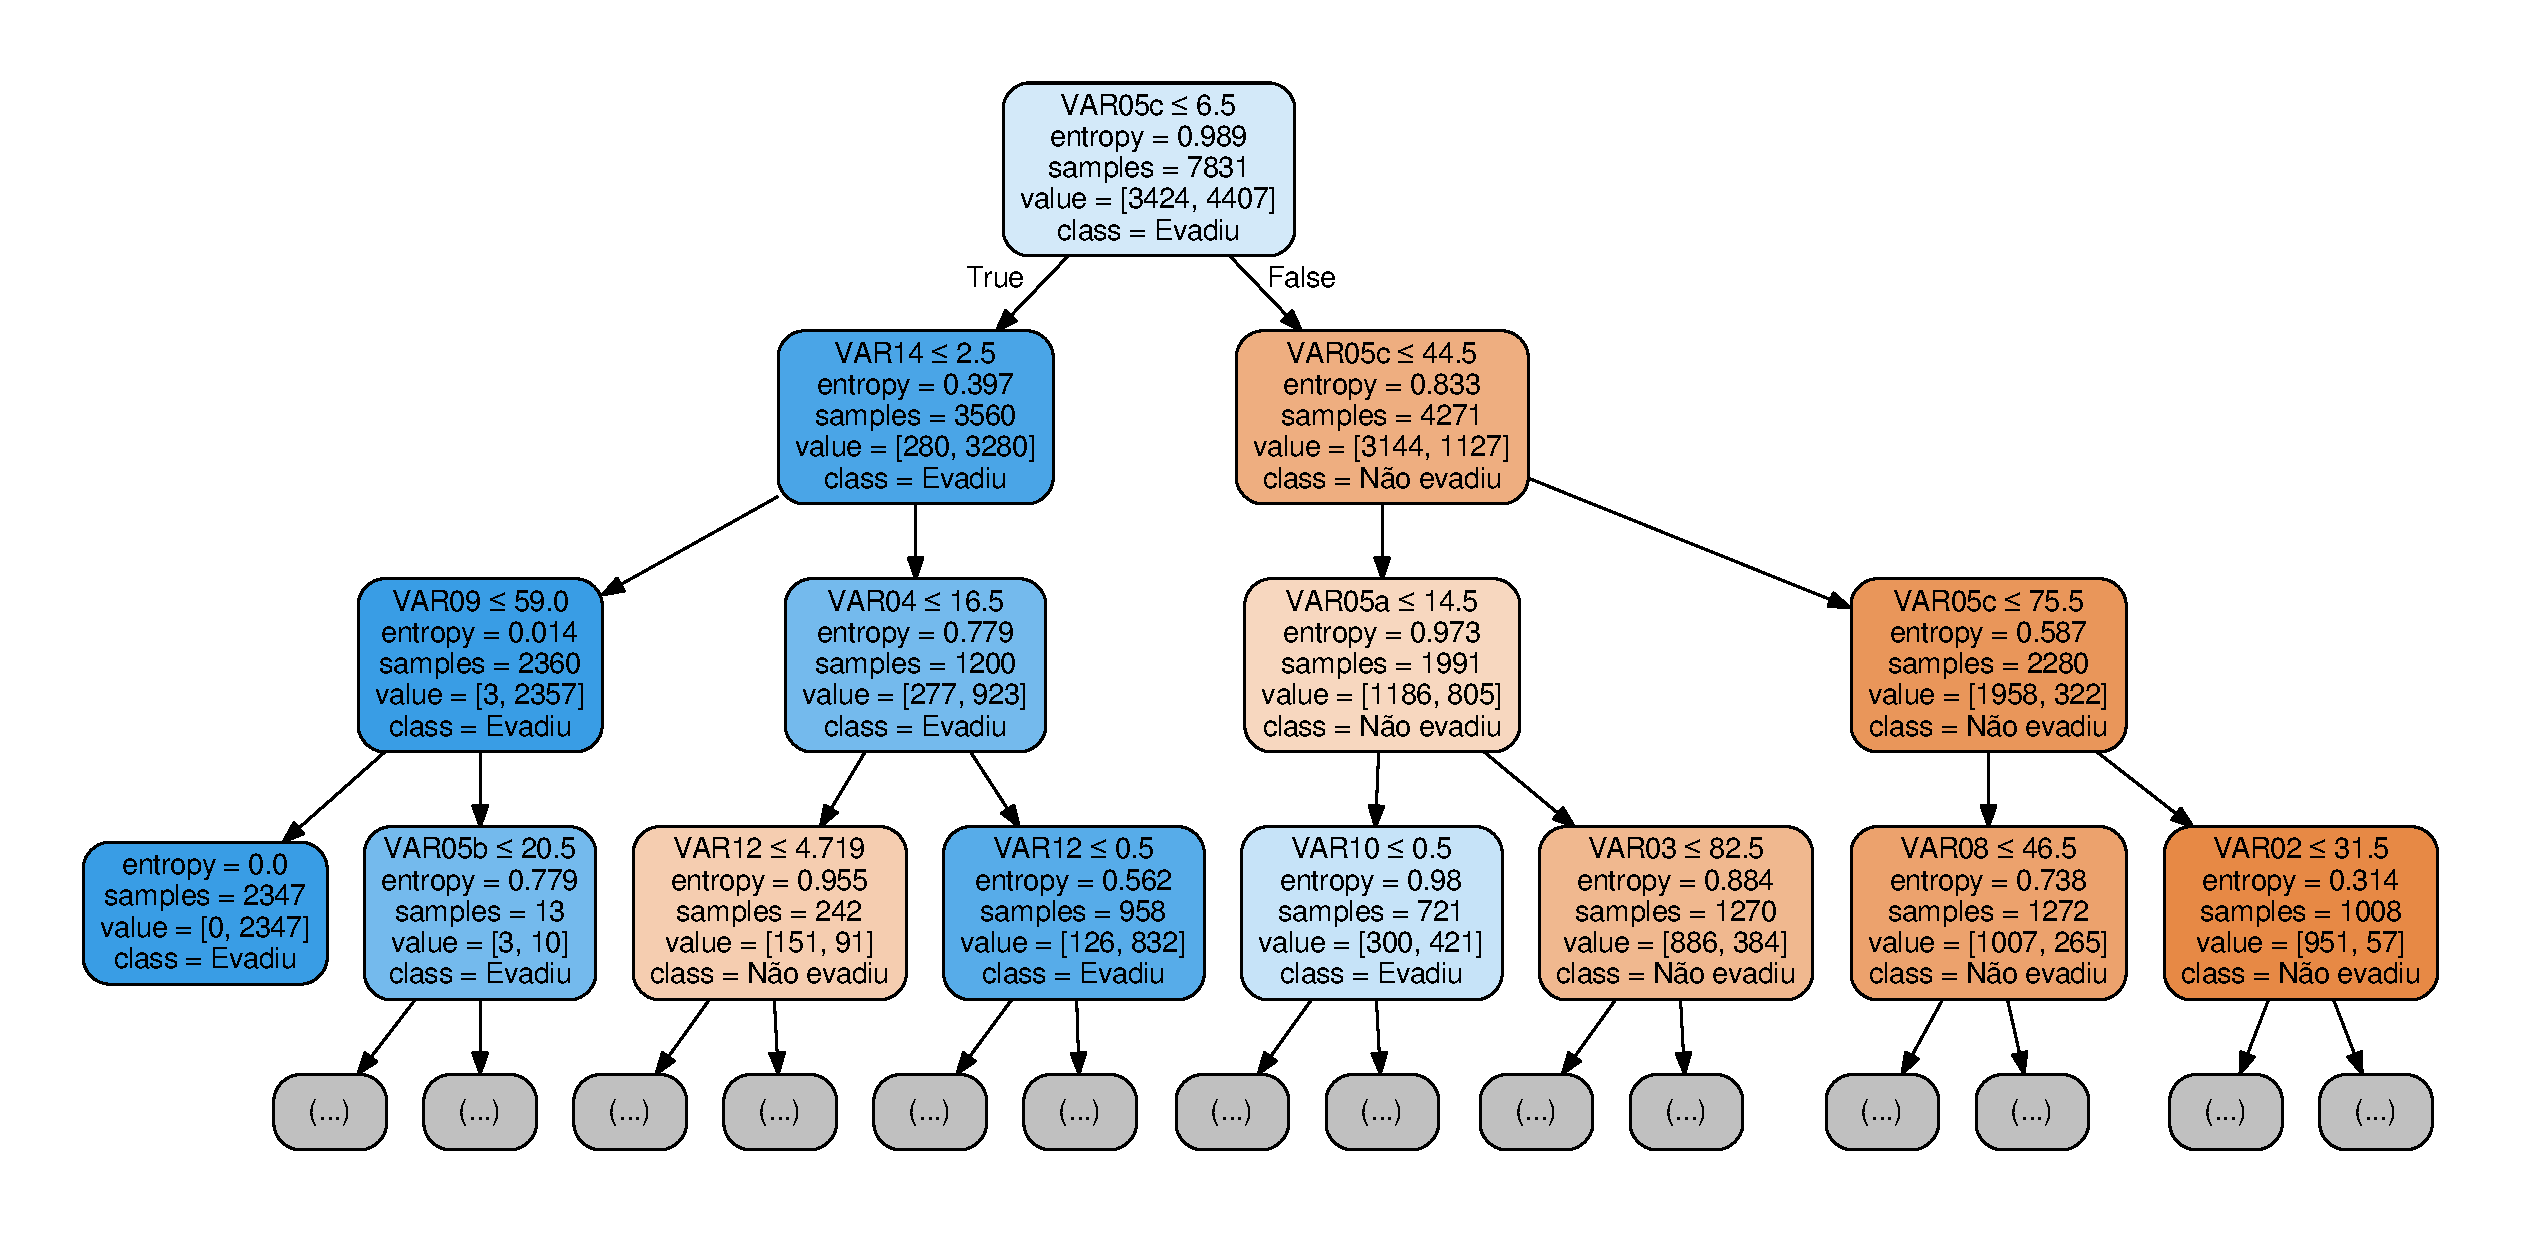
\includegraphics[angle=-90,scale=.50]{img/adm_tree_no_var07}
  \Ididthis
\end{figure}

Nas novas árvores, a variável com maior importância foi a \textit{VAR05c}, que
representa a quantidade de acessos do aluno ao ambiente no período da noite, por
semestre.

\section{Pós-processamento}

Os dados foram convertidos para formato CSV de forma que podem ser utilizados no
futuro para treinamento ou validação de outros algoritmos de classificação.

Os  scripts e visualizações geradas foram disponibilizadas publicamente em um
repositório público.

\section{Conhecimentos Obtidos}

A análise dos dados permitiu perceber que os alunos da EAD na UNIVASF tendem a evadir entre o quarto e quinto semestre do curso.

Os algoritmos de classificação apresentaram métricas compatíveis com as encontradas na literatura.

Para o curso de Licenciatura em Pedagogia, o algoritmo Árvore de Decisão foi o
que obteve as melhores métricas, com exceção da sensibilidade, onde ele ficou
abaixo do KNN. A variável com maior importância, segundo o gráfico da árvore,
foi a \textit{VAR07} seguida pelas \textit{VAR04}, \textit{VAR08} e
\textit{VAR14}.

O mesmo comportamento foi observado para o curso de Bacharelado em Administração
Pública.
O fato da Variável \textit{VAR07} (Quantidade de acessos do aluno ao ambiente no semestre - Autonomia),
ter sido destacada como mais importante em ambos os cursos é explicado pelo fato da mesma a variável que define a principal
característica de um aluno evadir-se ou não, afinal sem acessar o ambiente virtual, nenhum recurso
pode ser visualizado e nenhuma atividade pode ser executada, nenhum comportamento do aluno pode ser verificado, além do baixo
ou nenhum acesso aos cursos.
Além disso, o fato da mesma apresentar uma grande variabilidade em seus valores, pode também ter
influenciado nessa importância em relação às demais.

\section{Considerações Finais do Capítulo}

Neste capítulo foram apresentados os resultados obtidos em cada etapa do KDD
aplicada neste trabalho, foi verificado a distribuição das classes nos conjuntos
de dados, as estatísticas descritivas das variáveis, as métricas dos algoritmos
de classificação e as visualizações das árvores de decisão.

No proximo capítulo, serão apresentadas as considerações finais desta pesquisa e
sugestões de trabalhos futuros.
